\documentclass[output=collectionpaper]{langsci/langscibook}

\title{The feminine anaphoric gender gram, incipient gender marking, maturity, and extracting anaphoric gender markers from parallel texts}
\shorttitlerunninghead{The feminine anaphoric gender gram}

\author{%
Bernhard Wälchli
\affiliation{Stockholm University}%
}%

% \chapterDOI{} %will be filled in at production

\abstract{%
\label{firstpage:Waelchli}
The aim of this paper is to carry out a typological study of feminine anaphoric gender grams (such as English \textit{she/her}) in a large world-wide convenience sample of 816 languages and based on a strictly procedural definition. The investigation pursues a radically functional approach where the functional equivalence of the forms under study is assured by exploring an identical search space in parallel texts (translations of the New Testament) in all languages of the sample. This is the first large scale typological study of grammatical gender based on parallel texts, and a large part of the paper is devoted to methodological aspects. The study shows that gender has a functional core like any other grammatical category, and that it can at least partly be studied without resort to the notions of noun class, agreement and system. The results show that a large number of languages possess simple forms of gender, often representing incipient gender from a grammaticalization perspective. The paper discusses how simple gender differs from more mature and genealogically more stable forms of anaphoric gender. Finally the feminine anaphoric gram type is considered in its wider context, reconciling it to the traditional global approach focusing on the notions of system, noun class and agreement.
\medskip

\textbf{Keywords:}
feminine gender, anaphora, anaphoric pronouns, grams, grammaticalization, grammatical relations, functional domains, constructional islands, cue validity, maturity, parallel texts
}%

\maketitle
\begin{document}

\section{Introduction}
\label{sec:BW:1}

The traditional definition of gender (“Genders are classes of nouns reflected in the behavior of associated words”; \citealt[231]{Hockett1958}) rests on the notions of noun class and agreement. With the exception of classifiers, for which noun classes are crucial as well, these notions do not figure in the definitions of other grammatical categories. This makes gender stand out among grammatical categories as very specific by definition. In this paper it is argued that it is also possible to address gender as any other grammatical category by defining it as “Grammatical category expressing meaning X”, where X can be feminine, masculine, animate and inanimate, given that the most widespread meanings in gender are animacy and sex (\citealt[101]{Dahl2000a}; \citealt[68]{Corbett1991}; \citealt{Luraghi2011}), at least as far as anaphoric gender is concerned.%
\footnote{%
One of the first things I was ever taught in linguistics is that gender and sex are absolutely not the same thing and, since my department found me highly suitable for teaching numerous courses in discourse studies, sociolinguistics, and pragmatics and intercultural communication, I am quite familiar with gender studies and the notion of performative gender. However, the approach pursued in this paper focuses exclusively on the semantic core of feminine and masculine grammatical genders and here the gross simplification that sex is the core meaning of masculine and feminine gender grams has proven to be very useful in practice.
} %
In order to make clear that this paper mainly deals with gender marking in anaphoric contexts, I will use the term “anaphoric gender”. The question of how grammatical gender is defined is highly relevant for assessing the complexity of grammatical gender.

Noun classes and agreement are complex phenomena. Accepting the traditional definition of gender as the only option would mean to take for granted that grammatical gender is complex by definition. In order to assess the complexity of grammatical gender empirically it is indispensable to explore the possibility of simpler alternative definitions. Linguists nowadays often understand “gender” and “noun class” as full synonyms. This may be appropriate for the study of gender within noun phrases, but does not do justice to the use of gender in the anaphoric domain, which is the topic of this paper.

The major aim of this paper is to show that gender has a functionally motivated semantic core that can be considered in abstraction from the notions of noun class and agreement. This is done by formulating a procedural definition of feminine anaphoric gender which is so explicit that it can be implemented in a computer program in order to extract certain feminine gender markers from parallel texts (here translations of the New Testament). Feminine is chosen for practical reasons. It is easiest to address in this particular corpus (see \sectref{sec:BW:2.2}).

The underlying idea is that grammatical categories can be captured in terms of \spterm{grams}. A gram is a grammatical item in a particular language with specific form and specific meaning and/or function (\citealt{Bybee1989}; \citealt{Dahl2016}). Grams can be considered in abstraction from the language-specific systems they are part of. For instance, perfect and progressive can be investigated in abstraction from tense and aspect systems. For gender grams this means that the units of research are feminine, masculine, animate and inanimate, rather than gender systems. Virtually all gender systems are sensitive to the meanings sex and/or animacy (whereby different segments of the animacy hierarchy can be affected). It is true that gender in many languages also comprises other meanings, such as size and shape, and these other meanings are very important for the study of gender as systems. With the gram approach, however, it is possible to address the semantic core areas and to study them cross-linguistically, without having to consider the entire gender systems. A strength of the gram approach is its selectivity. Only salient semantic core uses are considered and compared cross-linguistically. A gram necessarily has a semantic core, but not all of its uses need be semantically motivated. The gram approach focuses on the semantic core of grammatical categories and investigates to what extent grams across different languages share their semantic core, put differently, cluster to cross-linguistic gram types. In order to find out whether a language has a gram reflecting a cross-linguistic gram type, it is sufficient to consider the prototypical uses of a gram type.

Focusing on the semantic core means focusing on those uses of a grammatical category where it is most transparent semantically. We know, among other things, from Corbett’s (\citeyear{Corbett1991}, chap.~8) study of the Agreement Hierarchy that gender use tends to be most transparently semantic in third person anaphoric pronouns. According to \citet{Audring2009a}, all pronominal gender systems (where gender is restricted to pronouns) are semantically organized, which further supports the view that gender is most semantic in anaphoric use.

A feminine gender gram \textendash{} in its prototypical use \textendash{} is a grammatical element picking up reference to a female human, such as the English third person singular pronominal forms \textit{she} and \textit{her} exemplified in (\ref{ex:BW:1}). (\ref{ex:BW:1}) is one of 74 parallel corpus passages that are used as a search space for feminine anaphoric gender grams in this paper.

\ea\label{ex:BW:1}
English (Indo-European; Matth.~15:26--27): gender marking on free pronouns\\
\textit{But he answered: ``\ldots'' But \textbf{she} said: ``\ldots''}
\z

What I have said so far may suggest that this is a paper about gender in personal pronouns such as English \textit{she} (see, e.g., \citealt{Audring2009a}), but the search space is much broader. In many languages the functional equivalent to she and her in English is an affix on verbs and/or adpositions as in (\ref{ex:BW:2}) from Garifuna.

\ea\label{ex:BW:2}
Garifuna (Arawakan; Matth.~15:26–27): gender marking on bound pronouns and prepositions\\
\gll Ába	\textbf{l}-aríñagun	Jesúsu	\textbf{t}-un:	``\ldots''	Ába	\textbf{t}-aríñagun:	``\ldots''\\
and	3\textsc{sg.m}-say	Jesus	3\textsc{sg.f}-to {}		and	3\textsc{sg.f}-say {}\\
\glt ‘But he answered: ``\ldots'' But she said: ``\ldots'' ’
\z

Third person pronouns and affixes for third person have in common that they are \spterm{reduced referential devices} in terms of Kibrik (\citeyear{Kibrik2011}; ch.~3), who calls them \spterm{free} and \spterm{bound pronouns}. In (\ref{ex:BW:1}) from English the gender marking is located in free pronouns, but in (\ref{ex:BW:2}) from Garifuna and (\ref{ex:BW:3}) from Ama it is in bound pronouns (pronominal affixes). While Garifuna has bound pronouns indexing subject, Ama has bound pronouns indexing absolutive (S, O and R[ecipient]). Hausa in (\ref{ex:BW:4}) marks pronominal gender mainly on aspect words, a kind of auxiliary that is preposed to the verb, but also has optional free pronouns.

\ea\label{ex:BW:3}
Ama (Arai/Left May; Matth.~15:26–27): gender marking on bound pronouns (S, O only)\\
\gll [\ldots]	no-na-ni	imo	na	i-\textbf{so}-ki,	Isiso	mo. Ulai	no-na-ni	nukonu	mo	na	\textbf{imo}-ki,	``\ldots''\\
{} that-\textsc{foc}-here	talk \textsc{foc}	say-\textsc{o.3sg.f-rem.pst}	Jesus	\textsc{top} but	that-\textsc{foc}-here	woman.\textsc{spec}	\textsc{top}	\textsc{foc}	say[\textsc{o3sg.m}]-\textsc{rem.pst}\\
\glt ‘But he answered (``\textbf{to her}''): ``\ldots'' But she said (``\textbf{to him}''): ``\ldots'' ’
\z

\ea\label{ex:BW:4}
Hausa (Afro-Asiatic; Matth. 15:26–27): gender marking on aspect words\\
\gll \textbf{Ya}	amsa	\textbf{ya}	ce:	``...''	Sai	\textbf{ta}	ce:	``...''\\
\textsc{3sg.m}	answer	\textsc{pst.3sg.m}	say		then	\textsc{pst.3sg.f}	say\\
\glt ‘But he answered: ``...'' But she said: ``...'' ’
\z

However, even if we consider affixes on verbs to be bound pronouns following Kibrik, the search space is not restricted to pronouns. Many languages have anaphoric forms intermediate between nouns and pronouns, for which I will use the name ``\spterm{grammatical anaphor}'' in want of a better term. Third person pronouns are, of course, also grammatical and anaphors, but since pronoun and third person pronoun are established terms, there is little risk of confusion. A grammatical anaphor is illustrated in (\ref{ex:BW:5}) from Kiribati. Kiribati has a personal pronoun not distinguishing gender (\textit{e} \textsc{3sg}), but there is also the “person demonstrative” (\citealt[176]{Trussel1979}) \textit{neierei} ‘that woman’, which is a noun phrase and displays the word order of a full noun phrase (VOS), but is different from the full demonstrative noun phrase \textit{te aine arei} [\textsc{art} woman \textsc{dem.dist}] ‘that woman’ and does not contain the noun \textit{aine} ‘woman’. Kiribati \textit{neierei} (70 times in the N.T.\@) mostly translates to ‘she’ and can also pick up reference to \textit{teinaine} ‘girl’ and \textit{tina-} ‘mother’ whereas \textit{te aine arei}
(13 times) [\textsc{art} woman \textsc{dem.dist}] translates to ‘the woman’.

\ea\label{ex:BW:5}
Kiribati (Austronesian, Micronesian; Matth. 15:27): grammatical anaphor\\
\gll Ao 	e 	taku 	\textbf{neierei}		... \\
and 	\textsc{3sg} 	say 	\textbf{that[\textsc{dist}].woman} \\
\glt ‘But she said: ``\ldots'' '
\z

Grammatical anaphors, such as Kiribati \textit{neierei} ‘that[\textsc{dist}].woman’, are less grammaticalized than pronominal gender markers such as English \textit{she}. Grammatical anaphors tend to be \spterm{incipient gender markers}, nouns on their way to be grammaticalized to pronominal indexes.

One possibility of interpretation is to argue that pronominal gender is more \spterm{mature} than non-pronominal gender in anaphors. Mature phenomena imply some sort of non-trivial historical development (\citealt[2]{Dahl2004}; \citealt{Trudgill2011}). Pronouns often differ from nouns in being suppletive according to grammatical relation. English \textit{she} (subject) and \textit{her} (object, indirect object, possessor) illustrate this point. Nouns are not entirely precluded from suppletion according to grammatical relation, but such suppletion in nouns is rare. Free and bound pronouns, however, usually display some sort of suppletion and/or neutralization according to grammatical relation. In Ama (\ref{ex:BW:3}), gender is distinguished in S, O and R, but not in A. Suppletion or neutralization in pronouns can be viewed as a feature of complexity and a feature of maturity.

Another possible interpretation is that gender cumulating with case (grammatical relation), as it often occurs in free and bound pronouns, is a different kind of phenomenon. \citetv{Waelchlithisyeara} argue following \cite[142]{Nichols1992} that agreement (and notably agreement in case and number) often triggers noun classification rather than vice versa. Put differently, at least in some instances, gender originates from case, and gender then tends to exhibit particular cumulation patterns with case from its very origin. While, following the second interpretation, cumulation and/or neutralization in certain grammatical relations might be incipient within gender, it is still mature in the sense of grammaticalization, as the development of gender then draws on preexistent grammatical categories (case, number and person).

In this paper I will extract feminine gender grams from translations of the New Testament (N.T.). Translations of the N.T.\ are parallel texts, and parallel texts allow us to define a semantic core in a very simple manner as a set of aligned passages. The N.T.\ comes segmented in chunks slightly larger than sentences (so-called verses), which is why no sentence alignment has to be made. The N.T.\ is translated into many languages and many translations are available electronically. Working with unannotated translations from many languages has the advantage that larger samples than usual can be used and that the dependence on individual grammar writers’ reporting or not reporting relevant characteristics is reduced. The most important advantage, however, is that working with automatic extraction forces us to formulate a fully explicit \spterm{procedural definition} of the wanted category, which is then applied in exactly the same way to all languages considered. In particular, the heuristic potential of automatic extraction is invaluable. The automatic device is naive and does not have any preconceived opinions about what kinds of markers should be included or not. In this particular study, this has helped me find various non-mature gender grams which have been overlooked in the gender literature so far, such as Kiribati (\ref{ex:BW:5}).

The procedural definition of the feminine gender gram will be discussed in more detail in \sectref{sec:BW:2}. It has essentially two components: (a) finding markers associated with a semantic core in a \spterm{functional domain} (\citealt{Givon1981}) and (b) filtering out markers which are also associated with other semantic cores (notably masculine gender and female light nouns such as ‘woman’, ‘girl’ and ‘mother’). Despite differences concerning parts of speech (pronouns, verbs, auxiliaries) and grammatical relations (A, S, R, O) exhibiting or not exhibiting feminine gender, all languages exemplified in (1--5) mark feminine gender in the same context in the parallel text corpus. The markers all occur in the same functional domain. Nothing in the procedural definition is in any way related to the notions of noun class and agreement. This means that if the endeavor is successful, it is possible to define feminine anaphoric gender grams in abstraction from the notions of noun class and agreement.

What does all this mean for the understanding of gender? Corbett’s Agreement Hierarchy is evidence that there is a semantic pole (anaphors) and a syntactic pole (NP-internal agreement) in gender. Traditional research focusing on noun classes and syntactic agreement considers the syntactic pole to be basic. This culminates in the Canonical Approach to gender, which focuses on gender values of nouns and considers redundant gender marking and local agreement domains to be canonical (\citealt{Corbett2016}). In this paper I argue that a shift of perspective is possible where semantic and referential gender in anaphora is the primary concern of grammatical gender, whereas syntactic, lexical and redundant gender is secondary.

The following sections are structured as follows. \sectref{sec:BW:2} motivates and formulates the procedural definition of the feminine anaphoric gender gram and \sectref{sec:BW:3} discusses its practical implication in the parallel text corpus and reports the results. \sectref{sec:BW:4} elaborates on the distinction between mature and non-mature grams and how it is related to grammatical relations. \sectref{sec:BW:5} focuses entirely on those non-mature gender grams that are non-pronominal and arguably incipient anaphoric gender markers. Finally, \sectref{sec:BW:6} discusses how the functional approach developed in this paper can be connected to the traditional system perspective on gender and \sectref{sec:BW:7} concludes this paper.


\section{A procedural definition of the feminine anaphoric gender gram}
\label{sec:BW:2}

\subsection{Overview}
\label{sec:BW:2.1}

This paper focuses on a domain where gender is most obviously used semantically and which is easiest to address by automatic extraction in the N.T.\ corpus. In \sectref{sec:BW:2.2} I am going to discuss why feminine is easiest to address. I will then discuss why feminine anaphoric can be viewed as a functional domain which can be defined as a set of passages in the parallel text corpus (\sectref{sec:BW:2.3}). The next step is to discuss what makes markers of feminine gender differ from other markers closely associated with the feminine anaphoric functional domain (\sectref{sec:BW:2.4}). This will allow us to formulate a procedural definition of the feminine gender gram which is sufficiently elaborate for the purposes of this paper. Finally, based on the notions of cue validity and constructional islands, \sectref{sec:BW:2.5} discusses why anaphoric gender grams in most languages are accessible without previous familiarity with the entire language system.

\subsection{Why feminine, why singular and why anaphora?}
\label{sec:BW:2.2}

We know from Corbett’s Agreement Hierarchy that the semantically most transparent use of gender is found in third person anaphoric pronouns. However, this does not mean that grammatical gender has the function of reference tracking in discourse.%
\footnote{%
According to Kibrik gender is used as a deconflicter in reference tracking in an “opportunistic way” \citet[359]{Kibrik2011}. Languages rely on referential aids to various extent and some languages without gender such as Navajo (Na-Dene) are more strongly inclined to use reduced referential devices than some languages with gender such as Archi (Nakh-Daghestanian) (\citealt[336]{Kibrik2011}).
} %
Within anaphoric use, the descriptive content of gender is most active in contrastive use in implicit or explicit focus (\citealt[227]{Bosch1988}; \citealt[25]{Seifart2018}), and contrastive use (‘but she’) is represented in the clauses selected for the extraction from the corpus as in (\ref{ex:BW:1}). Since gender is often neutralized in the plural (even though this is no strict universal, see \citealt{Plank1997}), the search space is restricted to singular. The most widespread meanings in gender grams are animacy and sex. Sex is easier to identify than animacy, since animacy comes in many different forms in grammatical markers, not only as gender feature, but also as condition on gender (\citealt{Corbett2006}, chap.~6) and is, among other things, also involved in the choice of case or adposition in differential object marking (\citealt[166]{Croft2003}). This leaves us with masculine (singular) and feminine (singular) as possible choices. In the N.T.\ corpus, feminine is the much easier choice. Reference to male beings is strongly overrepresented in this text, which makes it difficult to distinguish between third person masculine and third person in general in automatic extraction. A further complication in this particular text is that the distinction between male and deity is fuzzy, which, in many languages, calls for specific solutions where this distinction is relevant in grammar. Thus, feminine singular in the anaphoric domain is clearly the easiest option to choose.

\subsection{Feminine anaphoric as a functional domain}
\label{sec:BW:2.3}

Defining feminine anaphoric gender as a functional domain in parallel texts means identifying a set of passages where this function is expressed recurrently across all translations of the text. Such a passage is Matthew 15:27, which has been illustrated from various languages in Section 1 and which is for convenience repeated here in English in (\ref{ex:BW:6}).

\ea\label{ex:BW:6}
English (Indo-European; Matth.~15:27)\\
\textit{But \textbf{she} said: ``\ldots''}
\z

Saying that (\ref{ex:BW:6}) reflects the feminine anaphoric functional domain abstracts from the fact that this passage is related to another passage earlier in the text given in (\ref{ex:BW:7}). In (\ref{ex:BW:7}), the referent of the anaphor in (\ref{ex:BW:6}) is introduced in the form of an indefinite noun phrase.

\ea\label{ex:BW:7}
English (Indo-European; Matth.~15:27)\\
\textit{And behold, \textbf{a Canaanitish woman} came out from those borders\ldots}
\z

Another way to put it is that anaphors tend to be coreferent with full noun phrases introduced earlier in the text, which is not strange given that anaphora “is the phenomenon whereby one linguistic element, lacking clear independent reference, can pick up reference through connection with another linguistic element” (\citealt[379]{Levinson1987}). However, this does not mean that all anaphora have explicit antecedents with which they are exactly coreferent, as illustrated in (\ref{ex:BW:8}).

\ea\label{ex:BW:8}
Anaphors without explicit antecedent (\citealt[98]{Hintikka1985}):\\
\textit{A couple was sitting on a bench. \textbf{He} stood up and \textbf{she} followed \textbf{his} example.}
\z

Not only pronouns, but even full NPs can be used in anaphoric function, and third person pronouns and full NPs have very similar properties in anaphoric function as shown, in (\ref{ex:BW:9}). Pronominal anaphors and definite NPs can both be used to make attributions of gender and neither of them requires a syntactically explicit antecedent, but they are both definite expressions.

\ea\label{ex:BW:9}
Pronouns and full NPs in anaphoric function (\citealt[98]{Hintikka1985}):\\
\begin{xlist}
\ex
\textit{The teacher addressed the children. \textbf{He/The man} was stern.}
\ex
\textit{A couple was sitting on a bench. \textbf{He/The man} stood up and \textbf{she/the woman} followed \textbf{his/the man’s} example}
\end{xlist}
\z

However, when assembling a set of passages expressing feminine anaphoric in a parallel text corpus, it is possible to abstract from the fact that most anaphors have NP antecedents and that a lexical item in the NP can determine the gender value in a way that goes against the core meaning of gender.



\subsection{Filtering out markers of feminine gender grams from the feminine anaphoric functional domain}
\label{sec:BW:2.4}

All languages have some anaphoric expressions in the feminine anaphoric domain, but not all expressions are grammatical expressions and not all grammatical expressions are feminine. The anaphoric expressions in the feminine anaphoric domain can be nouns, such as ‘woman’ or ‘girl’, or they can be pronouns not distinguishing gender. This is both illustrated in (10) from Turkish with the noun \textit{kadın} ‘woman’ and the general third person pronoun \textit{o} ‘he/she’.

\ea\label{ex:BW:10}
Turkish (Matth. 15:24–27)\\
\gll \textbf{İsa}, «\ldots»	diy-e	cevap	ver-di.	Kadın	ise	yaklaş-ıp, «\ldots»	diyerek [\ldots]. İsa	o-na, «\ldots»	de-di.	Kadın, «\ldots»	de-di. «\ldots»\\
Jesus	{} say-\textsc{cvb}	answer	give-\textsc{pst3}	woman	however	approach-\textsc{cvb} {} say-\textsc{cvb} {} Jesus	\textsc{3sg-dat} {}	say-\textsc{pst3}	woman {}	say-\textsc{pst3} {}\\
\glt ‘But \textbf{he} [=Jesus] answered and said, “\ldots” But \textbf{she} [=the woman] came [\ldots] saying, “\ldots”. And \textbf{he} [=Jesus] answered (to \textbf{her}) and said, “\ldots”. So \textbf{she} [=the woman] said, “\ldots” ’
\z

It is thus not all expressions in the functional domain of picking up reference to female humans that instantiate feminine gender. If we extract the forms which are associated with the feminine anaphoric domain, which can easily be done by means of collocation measures (see \sectref{sec:BW:3}), the recall will be too large. Put differently, many nouns, such as Turkish \textit{kadın} ‘(a/the) woman’, and general anaphoric pronouns, such as Turkish \textit{o} ‘he/she’, will be extracted as well. One way to account for this is to define the search domain very narrowly by excluding such contexts where many languages use nouns instead of pronouns. But cross-linguistic and stylistic differences in the use of nouns, pronouns and zero anaphors are so large that a restrictive search domain is not sufficient.

The solution which is chosen here is to filter out expressions such as Turkish \textit{o} ‘he/she’ and \textit{kadın} ‘(a/the) woman’. By subtracting forms associated with anaphoric masculine and anaphoric in general, we can make sure that none of the extracted forms is third person masculine or third person general. Expressions for ‘woman’ have their own functional domain, which only marginally overlaps with the feminine anaphoric. Notably they also contain non-anaphoric uses, such as (\ref{ex:BW:7}), where languages such as English have an indefinite article. Lexical nouns are not restricted to anaphoric uses, but can occur both in definite and indefinite uses. By subtracting all forms associated with the functional domain ‘(a/the) woman’ from the set of forms associated with the feminine anaphoric we can make sure that none of the extracted forms means ‘(a/the) woman’. The same procedure can be applied to a few other critical lexical domains, such as ‘girl’ and ‘mother’. Nouns are an open word class. Hence, the number of potential female lexical domains is potentially infinite. However, there is no need to care about rare lexical domains. It is sufficient to address the most frequent ones: ‘woman’, ‘girl’, ‘mother’, and ‘daughter’. This is sufficient for the particular parallel corpus used. If in another parallel corpus another female lexical domain would be particularly frequent, it would have to be included in the filter as well. Filters must be adjusted to particular parallel corpora. However, their content can be described in general terms in the procedural definition: “frequent female lexical domains”.

Filtering out all forms that might be associated with a lexical domain, we can also make sure that the remaining set of forms consists exclusively of grammatical markers. This does not restrict the set to pronouns. Grammatical anaphors, such as \textit{neierei} in Kiribati (\ref{ex:BW:5}), will still be included.

What has been said above, results in the procedural definition for feminine anaphoric gender grams given in (\ref{ex:BW:11}):

\ea\label{ex:BW:11}
Procedural definition of feminine anaphoric gender markers:\\
\begin{xlist}
\ex Extract all markers picking up reference to female humans
\ex unless they can also be used to pick up reference to male humans, and
\ex unless they express frequent female lexical domains (such as ‘woman’, ‘mother’, ‘girl’, and ‘daughter’)
\end{xlist}
\z

The concrete implementation of this definition is discussed in \sectref{sec:BW:3}.


\subsection{Constructional islands and cue validity}
\label{sec:BW:2.5}

The approach implemented in this paper rests on the assumption that markers expressing a grammatical or lexical meaning X can be viewed as constructional islands with high cue validity. I take these terms from the literature on first language acquisition (\citealt[113]{Tomasello2003}). In general terms, constructional islands can be defined as utterance-meaning pairings, where one part of the utterance, the marker, is constant, such as in the set: \textit{\textbf{more} milk}, \textit{\textbf{more} grapes}, \textit{\textbf{more} juice}. The marker has high cue validity, if it is sufficiently distinct from all other markers in the language and if it can be immediately recognized without any previous analysis of the morphology of a language, simply as a continuous sequence of sounds (a word form or a continuous segmental morph without allomorphs).

The notions of constructional island and cue validity can be directly applied to parallel text corpora, where a constant meaning can be defined as a set of passages in which a meaning is instantiated. In written corpora we have to take continuous sequences of characters instead of phonemes. All word forms and all continuous substrings of words are candidates for markers that are directly accessible without any previous analysis of the language system. Constructional islands with high cue validity can be detected in the corpus without any knowlegde about the structure of a language and without any resort to parts of speech, grammatical or lexical categories, paradigms or systems.

My assumption is that if a language has a feminine anaphoric gender gram, there will usually be at least one marker with high cue validity. Not all markers will have high cue validity, so the extraction will not be complete. But the approach will be sufficient in most cases for finding out whether or not the language has a feminine anaphoric gender gram. For this purpose, it is sufficient to find one marker if there is more than one.

Put succinctly, if there is no gram, no marker is detected, if there is a gram, at least one of its markers is extracted.

There may be languages where the cue validity of anaphoric gender grams is low, where gender is highly integrated in grammatical systems. These may be cases where the marker is short (just a single phoneme within words of a particular word class) and often neutralized or where the marker is zero (as opposed to a non-zero masculine marker). However, my assumption is that in the vast majority of languages, feminine gender grams have high cue validity and can be viewed as constructional islands, at least to some extent.


\section{Extracting feminine gender grams from parallel texts}
\label{sec:BW:3}

\subsection{Sample, data, and procedure}
\label{sec:BW:3.1}

The sample consists of 816 languages (listed in Appendix A and B) and is not stratified. It simply contains the languages for which I happened to have an electronic version of the New Testament available when I started this work, and, as in other work based on Bible translations, some areas, in particular North America and Australia, are strongly underrepresented. The texts are not annotated. Some texts which are not in Roman script have been Latinized, but differences in writing systems have very little impact on the extraction procedure. Where the writing system is relevant, this is discussed below. For a few languages, more than one translation has been used (a total of 858 texts). The differences within languages are not reported, since in most cases the results were largely constant within a language,%
\footnote{%
There are some minor differences as in German where the form \textit{ihr} [\textsc{3sg.f.dat}] is not extracted in some texts.
} %
but this does not change the fact that the translations represent particular varieties (doculects), and in a few cases there may be intra-language variety that has not been detected. In one case, Uduk, feminine anaphors have been deliberately created by missionaries (see \sectref{sec:BW:5.1}), but language planning is an issue only for few languages of the sample, which is why it is not excessively discussed in this paper.

While the theoretical notion of procedural definition of a category type (\ref{ex:BW:11}) is very general, there are several practical details in the extraction process that can be adjusted and must be adjusted (see below). As is usually the case in typological investigations, there is no gold standard. It is not known what the result is going to be before the investigation has been carried out. Hence, the automatic extraction must be complemented by an evaluation by means of grammars and other reference material. However, since grammatical gender is known to be genealogically stable in many language families, it was very useful to have a large number of languages from a few large families in the sample. I expected feminine anaphoric gender to be lacking in most languages of the following families: Austronesian (134 lgs.), Niger-Congo (127 lgs.), Trans-New Guinea (90 lgs.; except Ok-branch known to have gender), Quechuan (25 lgs.), Sino-Tibetan (24 lgs.), Uto-Aztecan (18 lgs.), Turkic and Uralian (17 lgs.), and to be present in most languages in the following families: Indo-European (50 lgs.; except for some Indo-Iranian languages and Armenian known to lack gender), Arawakan (17 lgs.\@) and Tucanoan (13 lgs.). This means that for roughly two thirds of the sample there was an expected result and the details of the extraction mechanism (set of verses included in the search space, filters, how to compare a filter with the search space, see below) could be adapted in a process of trial and error until the outcome largely matched the expected result. In practice, the most difficult thing was to avoid extraction of forms in languages without anaphoric gender grams, so it is very important that the sample contains a large number of such languages (Appendix B). This means that only about a third of the languages of the sample had to be checked manually with grammars and other reference material. Hence, due to its genealogical stability, gender is an exceptionally favorable domain for a typological investigation based on parallel texts with many languages.

In the course of investigation it then turned out that in several dozens of languages the results yielded other forms than just the expected third person free and bound pronouns even after the necessary practical adjustments in the algorithm. At closer introspection, it became clear that many of these languages had incipient anaphoric gender; put differently, anaphoric gender that is so simple that it has not figured prominently in the literature on gender so far, which traditionally focuses on complex cases of gender. This made it necessary to devote a large part of this paper to languages with incipient gender (\sectref{sec:BW:5}) and these languages also turned out to be typical exceptions to the expected genealogical stability of gender. The rest of the unexpected forms could be accounted for as various types of systematic errors due to the naive mechanic nature of the extraction algorithm (\sectref{sec:BW:3.3}).


\subsection{Extract all markers picking up reference to female humans}
\label{sec:BW:3.2}

The starting point for the extraction of feminine gender from the N.T.\ parallel corpus is the procedural definition in (\ref{ex:BW:11}).

First, the algorithm extracts markers picking up reference to female humans, based on collocation with a set of contexts where feminine anaphoric gender occurs.

In parallel texts meaning can be equated with a set of contextually embedded situations where the markers encoding that meaning (which are language-particular form classes) are expected to occur (\citealt[672]{Waelchli2012}). In order to identify the situations across translations into different languages, the texts must be aligned with each other on a level coming close to sentences (sentence alignment). The N.T.\ is aligned in verses and verses are often somewhat larger than sentences, but verse alignment comes close to sentence alignment. Extraction is much easier if the texts are also word-aligned, but here I use only verse alignment which is a crude approach.

For the sake of simplicity it is assumed that a marker is either a word form or a morph (a continuous part of a word form; in concrete terms, any continuous sequence of characters in a word form). This makes it possible to explicitly define the set of potential markers as all word forms and all continuous sequences of characters within word forms.

The easiest way to design a search domain is to take one or several \spterm{seed grams} (\citealt{Dahl2016}), forms from particular languages where it is known that they more or less accurately instantiate a gram. Such forms are the third personal singular feminine personal pronoun forms in English (\textit{she/her}) or in Scandinavian languages (Swedish \textit{hon/henne/hennes}). The English forms \textit{she} and \textit{her} occur together in 292 verses in the N.T.\ (American Standard translation). An extraction of potential markers is nothing else than a list of the word forms and character sequences (approximating morphs) that collocate best with the search space above a certain threshold with an appropriate collocation measure. If these 292 verses are used as a search space, an extraction of collocating forms will contain many of the wanted markers, but it will also contain many forms that should not be extracted (boldface in \tabref{tab:BW:1}).

\begin{table}
\begin{tabular}{lll}
\lsptoprule
  Language	&	Forms	&	Gloss of forms in boldface	\\
\midrule
  Turkish	&	\textbf{kadın}	&	‘woman’	\\
  Swedish	&	hon, henne, hennes, \textbf{kvinna}	&	‘woman’	\\
  English	&	her, she, \textbf{woman}	&	‘woman’	\\
  Koine Greek	&	αυτης, αυτη, >σα\#<, \textbf{γυνη}, \textbf{η}	&	‘woman’, \textsc{def.nom.sg.f}	\\
  Estonian	&	\textbf{naine}, \textbf{ta}, \textbf{tema}	&	‘woman’, \textsc{3sg}, \textsc{3sg.emph}	\\
  Tok Pisin	&	\textbf{meri}, \textbf{en}, \textbf{maria}	&	‘woman’, \textsc{3sg}, ‘Mary’	\\
  Indonesian	&	\textbf{perempuan}, >\textbf{nya\#}<	&	‘woman’, \textsc{poss.3sg}	\\
\lspbottomrule
\end{tabular}
\small{
\begin{flushleft}
Here and elsewhere the notation >x< will be used for morphs and \# is used for word boundaries.
\end{flushleft}
}%
\caption{Word forms and morphs best collocating with English \textit{she+her}}
\label{tab:BW:1}
\end{table}

A good extraction must meet two conflicting criteria. There should be as many correct extracted forms as possible (high recall), but there should also be as few wrongly extracted forms as possible (high accuracy). Since the majority of languages in the sample lack feminine gender grams, high accuracy is not as trivial as it might seem at first glance.

There are three ways improve accuracy: (i) We can use a higher threshold, but this is no good solution, since it has devastating effects on the recall. (ii) We can filter out wrongly extracted forms, since they can be grouped according to certain meanings which we can search for as well, such as ‘woman’ or general third person singular. (iii) We can reduce the search domain, so that the conflicting meanings are removed from it.

After many attempts I have decided to use a combination of (ii) and (iii). Probably it would be possible to work with the 292 verse search space and filtering, but I have not managed to design the filters such that the extraction is optimal. In the best attempt, there are in comparison to the extraction reported here wrongly extracted forms in 33 more languages and 10 languages are lost. The larger the search space, the more sophisticated the filters have to be. In larger search spaces there are simply more meanings represented and there is more that can go wrong.

In the extraction reported in this paper I have used a subset of 74 clauses as search space. The clauses have been selected manually, but more important than which clauses are selected is the simple fact that the set has about that size. If smaller sets are chosen it is increasingly more difficult to extract short bound morphemes, such a Garifuna >\#t-< in (\ref{ex:BW:2}). Explicit marking of word boundaries by a character makes peripheral morphs more salient and easier to extract.

The following criteria have been used to select the 74 clauses.

\begin{enumerate}[label=(\roman*)]
  \item Include verses where feminine anaphoric gender is instantiated several times, for instance, as in (\ref{ex:BW:12}):

  \ea\label{ex:BW:12}
  Two of 76 verses in of the trigger domain (given in the English Lexham translation)\\
42015009 (=Luke 15:9) And when \textbf{she} has found it, \textbf{she} calls together \textbf{her} friends and neighbors, saying, ‘Rejoice with me, because I have found the drachma that I had lost!’\\
44016015 (=Acts 16:15) And after \textbf{she} was baptized, and \textbf{her} household, she urged us, saying, “If you consider me to be a believer in the Lord, come to my house and stay.” And \textbf{she} prevailed upon us.
\z

  \item exclude long verses (where many other meanings are expressed);
  \item exclude clauses containing words for ‘woman’ in most texts;
  \item exclude most verses where feminine anaphoric gender is contrastive (‘but she’), because many texts have nouns for ‘woman’ there;
  \item exclude verses with ‘Mary’, so this proper name need not be filtered, and
  \item exclude (as far as possible) clauses with masculine anaphoric contexts (in fact, this cannot be strictly implemented, because masculine anaphoric contexts are omnipresent in the text).
\end{enumerate}

This results in a set of 74 verses%
\footnote{%
40001019 (i.e., 40 1:19 or Matth.\ 1:19; Matthew is the 40th book in the Bible), 40002018, 40008015, 40009025, 40012042, 40014008, 40014011, 40015023, 40015027, 40026012, 41005042, 41006024, 41006025, 41006028, 41007030, 41010004, 41014005, 41014006, 41014008, 42001029, 42001035, 42001036, 42001057, 42001058, 42001061, 42002006, 42002007, 42002036, 42002037, 42002038, 42007013, 42007035, 42007038, 42007047, 42008054, 42008055, 42008056, 42010040, 42010041, 42011031, 42013012, 42015009, 42018005, 42020031, 43004013, 43004016, 43004026, 43008005, 43011023, 43011033, 43011040, 43012007, 43019027, 43020014, 43020017, 44005008, 44005009, 44005010, 44009037, 44009040, 44012014, 44016015, 44016019, 44019027, 45007003, 45009012, 45016002, 46007028, 54005010, 58011031, 59002025, 66002021, 66002022, 66021011.
} %
two of which have been illustrated in (\ref{ex:BW:12}). Choosing the verse (or sentence/clause) as unit of alignment has an important consequences for the extraction of gender. It is not easily possible to distinguish between different grammatical relations, since the same verse often contains the feminine gender gram in various functions. This is notably true of reflexive possessors (as in \textit{she calls together \textbf{her} friends}) where even the clause is too large as a unit of alignment. Thus, the extraction applied here is not helpful in deciding which grammatical relation a marker encodes; only that it is some sort of feminine gender marker. The classification of markers according to grammatical relations in Appendix A has therefore been made manually with the help of reference grammars.

Furthermore, it needs to be pointed out that the N.T.\ is a text where feminine anaphoric gender is strongly underrepresented. Together with the considerable number of verses that have been excluded, this results in a quite small search domain, less than 1\% of the text. However, there are enough examples in the text for a mostly correct automatic extraction of frequent feminine gender grams, even if this sometimes means that only some, not all, markers of a feminine anaphoric gender gram are extracted. Extraction works quite well, despite the fact that the algorithm used here is crude. This testifies to the high cue validity of feminine gender markers. Put differently, in most languages identifying feminine gender grams is not particularly complex and does not presuppose any knowledge about gender systems.

The algorithm goes through all candidates and checks which of them matches best with the trigger domain according to a collocation measure (here T-score as defined by \citealt{Fung1994} is used) above a certain threshold. The threshold is determined empirically so that no or few incorrect forms appear. In order to demonstrate that this can be done in slightly different ways, two different thresholds have been applied: t=3.4 and t=3.19. The higher threshold prevents the first entirely wrong form to be extracted (Buglere \textit{chku} [arrive:\textsc{pfv}] ‘arrived’). However, with the higher threshold we also lose three languages with a feminine gender gram: Kabyle, Angami Naga and Owa (Owa is actually a borderline case, see 5.4), but there are also a large number of arguable errors among the 44 forms that are not extracted with the higher threshold. Since many errors are very interesting from a methodological point of view, I have chosen not to use only the higher threshold, which would probably have been the most reasonable thing to do for an optimal extraction. Forms only extracted with the lower threshold are given in curly braces in \tabref{tab:BW:2} and in Appendix A.

\begin{table}
\begin{tabularx}{\textwidth}{lll}
\lsptoprule
Language	&	Extraction	&	T-value of first form	\\
\midrule
Akateko (knj)	&	[ix]1	&	7.682	\\
Ama (amm)	&	[isoki]1	&	4.113	\\
Carapana (cbc)	&	[cõ]1 [>upo\#<]2 [>ñupõ\#<]3 [>mo\#<]4	&	7.738	\\
English (eng) [amstd]	&	[her]1 [she]2	&	7.2	\\
Garifuna (cab)	&	[>\#t<]1	&	6.008	\\
Hausa (hau)	&	[ta]1 [>ta\#<]2	&	5.309	\\
Kaingang (kgp)	&	[fi]1	&	7.636	\\
Latvian (lav)	&	[viņai]1 \{[>usi<]2 \}	&	4.152	\\
Owa (stn)	&	\{[kani]1 \}	&	\{3.191\}	\\
Zapotec, Miahuatlan (zam)	&	\{[xa\textquotesingle]1 \}	&	\{3.310\}	\\
\lspbottomrule
\end{tabularx}
\caption{Selected languages where feminine anaphoric gender markers have been extracted}
\label{tab:BW:2}
\end{table}

Although Indo-European languages have been the starting point for determining the distribution, it is rather languages from other families that have the best extraction values (the top three are Carapana \textit{cõ}, Kaingang \textit{fi} and Akateko \textit{ix} (see \tabref{tab:BW:2}).


\subsection{Filtering out conflicting meanings}
\label{sec:BW:3.3}

While the procedure described in \sectref{sec:BW:3.2} yields the correct result for most languages with anaphoric gender, the recall is too large in languages where anaphoric gender is lacking. The kind of forms wrongly extracted fall mainly into two semantic groups:

\begin{enumerate}[label=(\roman*)]
\item Indexes for third person singular not distinguishing gender. Forms expressing third person singular in general without making a gender distinction also collocate with feminine gender.
\item Words for ‘woman’, ‘girl/daughter’, and ‘mother’. This is surprising at first glance since most texts in Indo-European languages of Europe do not contain instances with ‘woman’ in the smaller search domain of 74 verses and too few for ‘girl/daughter’ and ‘mother’ to be extracted. These “errors” reflect the fact that many translations into languages without feminine anaphoric gender use words for ‘woman’ in contexts where languages with feminine gender use forms such as \textit{she} and \textit{her}, as in (\ref{ex:BW:10}) from Turkish. For determining whether a language has feminine anaphoric gender, the procedure must be refined so that such forms are not extracted.
\end{enumerate}

If forms collocating with the feminine third singular also include some forms for third person singular general and some forms for ‘woman’ and other general feminine nouns, extraction must take this into account by excluding forms which have a better correlation with third person singular masculine and with ‘woman’, ‘girl’ and ‘mother’.%
\footnote{%
To identify better correlations is not trivial since T-score values with larger search domains are generally higher than with small domains. Since there happen to be roughly two kinds of sizes of domains (smaller than 164 and larger than 742, see \tabref{tab:BW:3}), it is for practical reasons possible to apply a very crude solution by dividing all values of the larger domains by two before comparison. If this correction is not applied, a considerable number of feminine gender markers, for instance those in Kuot and Paumarí, are filtered out.
} %
The best way of doing this would be to define sets of verses for all conflicting meanings as carefully as for feminine anaphoric gender. Here, a cruder approach is used where these conflicting domains are simply represented by some characteristic instances in particular languages (\tabref{tab:BW:3}).

\begin{table}
\begin{tabular}{ll}
\lsptoprule
Masculine filter	&	English \textit{he} [2347 verses],	\\
(relates to (\ref{ex:BW:11}b))	&	English \textit{him} [1836 verses],	\\
	&	English \textit{he/him/his} [3570 verses],	\\
	&	English \textit{said to him} [164 verses]	\\
\padding
‘Woman’ filter	&	English \textit{woman} [54 verses],	\\
(\ref{ex:BW:11}c)	&	Xaasongaxango \textit{muso} ‘woman’ [39 verses]	\\
	&	Yau (yuw) \textit{owi} ‘woman, grandmother’ [1953 verses]	\\
\padding
‘Mother’ filter (\ref{ex:BW:11}c)	&	English \textit{mother} [76 verses]	\\
\padding
‘Girl’ filter (\ref{ex:BW:11}c)	&	Nalca \textit{gelma} ‘girl, daughter’ [40 verses],	\\
	&	Upper Pokomo \textit{mwanamuke} ‘girl’ [41 verses]	\\
\padding
‘Child’ filter	&	Tok Pisin \textit{pikinini} [743 verses]	\\
\lspbottomrule
\end{tabular}
\caption{Filters in the extraction of feminine gender grams}
\label{tab:BW:3}
\end{table}

\begin{enumerate}[label=(\roman*)]
\item \emph{The masculine filter}: For excluding general third person use, a form is not extracted if it correlates better with at least one of the following sets: (a) English \textit{he}, (b) English \textit{him}, (c) all uses of anaphoric masculine singular in English together (\textit{he}, \textit{him} and \textit{his}), and (d) all uses of \textit{said to him}. These four distributions all serve the same purpose, but conflicting forms can have different extensions, so all four of them are needed. Together they constitute the masculine filter.
\item \emph{The ‘woman’, ‘mother’ and ‘girl’ filters}: For the exclusion of lexical feminine meanings, a form is not extracted if it correlates better with at least one of the following sets: (a) the English singular form \textit{woman}, Xaasongaxango \textit{muso} ‘woman’, and Yau \textit{owi}, which is an instance of a very extensive use of a word for ‘woman’ occurring also in the co-compound \textit{owi amna} [woman man] ‘people’ (\citealt[104]{Sarvasy2014}), (c) English \textit{mother}, (d) Nalca \textit{gelma} ‘girl, daughter’, (e) Upper Pokomo \textit{mwanamuke} ‘girl’. This is to make sure that the basic meaning of an extracted form is not ‘woman’, ‘mother’ or ‘girl’ and only incidentally also occurs in the anaphoric domain. Several forms are needed since the semantic extension of words can vary (in some languages ‘daughter’ and ‘girl’ is expressed by the same word, in others by different words).
\end{enumerate}

After this is done, a smaller problem area remains which is presented here directly with the remedy resolving it:

\begin{enumerate}[label=(\roman*)]
\setcounter{enumi}{2}
\item
\emph{The ‘child’ filter}: In a few languages a word for ‘child’ is extracted. This is because children, child bearing, giving birth to children happens to collocate with the search domain in the N.T. This is solved by removing all forms that collocate better with Tok Pisin \textit{pikinini} ‘child’ than with the search domain. This is a practical complication that is so specific that I have not included it in the more abstract procedural definition in (\ref{ex:BW:11}).
\end{enumerate}

To paraphrase the whole procedure in a simple way: a feminine singular anaphoric gender marker is any form that collocates with the feminine singular anaphoric gender domain unless it rather means third person singular in general, ‘woman’, ‘mother’, ‘girl, daughter’, or ‘child’. Put differently, forms collocating with the feminine anaphoric singular gender must pass the masculine, ‘woman’, ‘girl’, ‘mother’ and ‘child’ filters before it is likely that they really represent the feminine anaphoric gender gram.

If the larger search space of English \textit{she+her} is used, further filters have to be added, notably ‘wife’, ‘husband’ and ‘Mary’ filters. There are also complex adjustments required for comparing T-score values with search spaces of different magnitudes.


\subsection{Unexpected extracted forms and whether they are errors}
\label{sec:BW:3.4}

Since there is no gold standard, extracted forms were checked with grammars and dictionaries. Checking revealed that after markers with conflicting meanings have been removed by filtering, there remain some unexpected extracted forms which could be considered errors. However, almost all “errors” are highly interesting in that they are somehow associated with the meaning of the feminine anaphoric gram. They fall into five types:

\begin{enumerate}[label=(\alph*)]
\item anaphoric (demonstrative or definite) forms of a word for ‘woman’,
\item demonstrative pronouns,
\item person name markers (determiners or titles), mostly female person name markers,
\item gender markers within noun phrases, and
\item the masculine gender form by female speakers,
\end{enumerate}

Finally, four occasional forms for ‘woman’, third person singular personal pronouns, and an entirely occasional verb form meaning ‘arrived’ escaped filtering with the lower threshold.

\begin{enumerate}[label=(\alph*)]
\item
\emph{Anaphoric (demonstrative or definite) forms of a word for ‘woman’}: In South Tairora the form \textit{nraakyeva} [\textit{nraakye-va} ‘woman-DEM’] is extracted, because the naive algorithm cannot recognize that it contains \textit{nraakye} ‘woman’ and should therefore be removed by the ‘woman’ filter. In South Tairora demonstrative NPs are formed by a free demonstrative, \textit{mwi}, \textit{mwa}, or \textit{mwatai} in the N.T.\ text, followed by a noun with an obligatory \textit{-va} suffix (\citealt[584]{Vincent2010}). The form \textit{nraakyeva} has the correct distribution since it only occurs in the feminine anaphoric domain; it is not a general form for ‘woman’ and passes therefore the ‘woman’ filter. This error thus derives from the fact that the algorithm applied here does not have the capacity to segment word forms into morphemes. Extracted forms with the same kind of error include Sabaot \textit{(:)cheebyoosyaanaa} ‘this woman’, Endo \textit{cheepyoosoonoonēē}, Ayautla Mazatec \textit{chjunbiu}, Safeyoka (Wojokeso) \textit{a'musi}, Umbu-Ungu \textit{ambomo}, and Rawa \textit{barega}
(see Appendix A IV). Several similar forms are slightly below the lower threshold for extraction, such as Low Tarahumara (\textit{muki-ka} ‘woman-\textsc{emph}') and Auhelawa (\textit{waihiuna-ne} woman-\textsc{dem/def}’). Also Ama \textit{nukonu} [woman.\textsc{spec}] (see (\ref{ex:BW:3})) sorts here, with an irregular form of the specifier (suffix \textit{-ta} in other nouns; \citealt[92]{Arsjoe1999}); however, this form is not extracted.

Generally, a demonstrative or definite form of ‘woman’ tends to be extracted whenever the demonstrative or definite marker is synthetic. This kind of error is particularly instructive because it shows us how anaphoric gender markers may emerge. Expressions for ‘that woman’ may qualify as anaphoric gender markers to the extent that the noun and demonstrative have become opaque. This is exactly what has happened in languages with non-compositional complex NPs such as Japanese (see  \sectref{sec:BW:5.2}). The errors made by the computer derive from the fact that more forms are opaque for the computer than for humans.

\item
\emph{Demonstrative pronouns}: Since complex expressions of ‘that/the woman’ are common feminine anaphoric expressions, it is not entirely unexpected that demonstratives and articles are occasionally wrongly extracted. This happens in several Trans-New Guinea languages: Mountain Koiali \textit{ke-u} [that-\textsc{subject}] (\citealt[428]{Garland1975}; in the N.T.\ in \textit{keate keu} ‘woman that’, \textit{ma keu} ‘girl that’), Folopa \textit{kale} ‘the’ (\citealt[85]{Anderson1989}; in \textit{kale so[-né]} ‘the woman[-\textsc{erg}]’), Fore \textit{kana-}
‘this mentioned one, the aforementioned’ (\citealt[45]{Scott1989}), and Awa \textit{mi} ‘that’ (\citealt{Lowing1975}) (Appendix A VI). I have not tried to add a demonstrative filter because demonstratives are too different in their distribution from each other and there is no point in adding filters that remove just one or two problematic cases.
\item
\emph{(Female) person name markers}: It is not uncommon for anaphoric gender markers to also be used together with person names. In a few languages the form is slightly different, thus Kiribati uses \textit{Nei} as a female person name marker and \textit{neierei} as anaphoric gender form. In North Halmaheran languages of the sample female names contain a form \textit{ngo}, which combines with the general determiner \textit{o}. A few languages in the sample have female person name markers but lack anaphoric gender. If the language at the same time happens to use many person names in the anaphoric domain, the person name marker can be wrongly extracted (Appendix A III). This is the case for Iraya \textit{bayi} (probably a shortening of \textit{babayi} ‘woman’), Uab Meto \textit{bi}, Satere-Mawe \textit{mana}, and Huave \textit{müm}.
\item
\emph{Gender markers within noun phrases are special cases of (b) and (c)}: demonstratives or extended person name markers that happen to bear NP-internal gender. In a sense these are not errors, since the forms mark feminine gender, but they mark feminine gender only NP-internally with common nouns and person names. This holds for Abau (\textit{sokwe} [\textsc{dist.dem.f.obj}]; \citealt[87]{Lock2011}), where there are also correctly extracted anaphoric forms, and for Kadiweu, Mocoví, and Nalca.

The Guaicuruan languages Kadiweu and Mocoví have so-called local classifiers (standing, sitting, lying, coming, going, absent; \citealt[62]{Sandalo1997}) in attributive demonstratives, which combine with masculine and feminine gender markers. In both languages only the form with the ‘going’ classifier is extracted: Kadiweu \textit{naɡ̶-a-jo} \textsc{close-f}-going and Mocoví \textit{a-so'-maxare} \textsc{f-going-pro} (Appendix A VI).

Nalca (Mek, Trans-New Guinean) has developed a gender system from person name markers (\citealt{Waelchli2018}), and the female person marker \textit{ge-} grammaticalized from \textit{gel} ‘woman’ has extended also to some female kinship terms and the word for ‘woman’. The extracted form is the topic form \textit{ge-ra} [\textsc{f-top}], which occurs in the search domain 15 times with female person names, 12 times with \textit{gel} ‘woman’ and twice with two different words for mother (Appendix A III). In the whole N.T.\ this form is only used once anaphorically, but not within the search domain.

It is not unexpected that some NP-internal non-feminine anaphoric gender forms, as in Abau, Kadiweu, Mocoví, and Nalca, are extracted by the algorithm, because, as far as anaphoric NPs occur in the search domain, they have the right distribution and are not filtered since they are both dedicated to feminine and non-lexical.

Some languages have derivational noun suffixes in female nouns, such as Parecis \textit{-halo}, Esperanto, and Iraqw  \textit{o'o} (\citealt[63]{Mous1992}). The Iraqw form is not extracted, the Esperanto form is eliminated by the ‘woman’ filter and the Parecis form is eliminated by the ‘girl’ filter.

\item
\emph{Masculine gender for female speakers and second person feminine}: Kayabi (Tupian) distinguishes both speaker and referent gender (see \sectref{sec:BW:4}). The verses of the search domain happen to contain a considerable number of quotations from female speakers which are basically useless for the extraction of the feminine gender gram. While the quotations do not do any harm for most languages, for Kayabi they cause with the lower threshold the error that \textit{kĩã} ‘\textsc{m 3sg} (female speaker)’ is wrongly extracted. Also due to direct speech in the search domain is the extraction of Mwaghavul \textit{yi}, a form for second person feminine reference, even this only with the lower threshold.
\end{enumerate}

Finally, the most problematic wrongly extracted forms are four forms that escaped filtering. But three of them are extracted only with the lower threshold t=3.19. One form for ‘woman’ Ama \textit{iní} ‘woman’ escaped filtering (Appendix A V). General third person pronouns in two Zapotecan languages were wrongly extracted (Appendix A VII). In Chichicapan Zapotec \textit{bi} is opposed to third person respect \textit{ba} (\citealt{Benton1975}) and escapes the masculine filter, probably because Jesus is referred to with the respect form. For Chichicapan Zapotec \textit{bi} even using the higher threshold does not help; the T-value is high (t=5.24). Miahuatlan Zapotec \textit{xa\textquotesingle} is another general anaphoric marker for third person (both masculine and feminine) that happens to have escaped filtering with masculine domains. These cases show that filtering is not always reliable, especially if forms for ‘woman’ and general third person singular deviate from their expected distribution in the text. Finally, as mentioned in \sectref{sec:BW:3.2}, Buglere \textit{chku} ‘arrived’ is the first fully unsystematic kind of error at t=3.39.

\subsection{Languages where the automatic extraction fails to detect gender}
\label{sec:BW:3.5}

Languages where gender is not extracted can be ordered into the following groups:

\begin{enumerate}[label=(\alph*)]
\item
There is agreement gender or there are noun classifiers reminiscent of agreement gender within the NP, but no or virtually no anaphoric gender: Limbu (\citealt[21]{Driem1987}), Baruya, Biangai, and Mopan Maya (\citealt{Contini-Morava2018}) (for Nalca, Kadiweu and Mocoví, see \sectref{sec:BW:3.4} above).
\item
Gender is distinguished in pronouns, but only in the second or in the second and first persons: Basque, Paez (\citealt[136]{Jung2008}, first and second person, but not third person) and Iraqw. However, in Mwaghavul some second person singular form \textit{yi} has been wrongly extracted, since second person with female referent often occur in direct speech in the search domain (see \sectref{sec:BW:3.4} (e)).
\item
There is feminine anaphoric gender, but it only covers the domain of girls or young women, the adult women domain is covered by a general human respect gender: Coatzospan Mixtec and Texmelucan Zapotec. These are removed by the ‘girl’ filter. The ‘girl’ filter is also responsible for eliminating the reduced nominal anaphor \textit{ta̱hn} in Teutila Cuicatec. In Tlalcoyalco Popoloca the anaphoric forms generally correspond to specific feminine lexemes and are therefore filtered out (see \sectref{sec:BW:5.3}) by the ‘woman’ and ‘girl’ filters. A more problematic case is Southern Puebla Mixtec, where the gender marker has many allomorphs (\textit{-nè}, \textit{-ne},  \textit{-né}, \textit{-ñá}, \textit{-ña} \textsc{f}), and the only one that is detected happens to be removed by the ‘woman’ filter.
\item
Gender marking is restricted to a limited part of the S and P domain and the markers do not have high cue validity: Chechen, Hindi, Gujarati, and Eastern Panjabi. These are languages with feminine genders, but the anaphoric function in those languages is marginal or non-existing. In Avar only gender on free pronouns is detected.
\item
The marker is partly zero as opposed to a non-zero masculine marker: This holds for the Arawakan languages Pajonal Asheninka, Ashaninka, Caquinte, Pichis Asheninka and Nomatsiguenga. The algorithm as implemented here is simply not smart enough for recognizing zero as the marker of the feminine gender gram. The recognition of zero morphemes requests some understanding of systems or at least oppositions.
\item
Gender is too inconsistently marked to be extracted: In Iraqw (Cushitic, Afro-Asiatic; \citealt{Mous1992}), masculine and feminine are not distinguished in third person free pronouns, and in affixes in verbs and auxiliaries, the markers are manifold both for the expression of subject and object (e.g., \textit{ó\textquotesingle} ‘she said’ vs.\ \textit{óo\textquotesingle} ‘he said’). It is not possible to detect feminine marking as constructional island without previous analysis of the paradigms. The algorithm fails to detect feminine anaphoric gender in Iraqw.
\item
The dominant marker is orthographically identical with another form: Teutila Cuicatec.
\end{enumerate}

The types (a) and (b) are no real errors since the algorithm only extracts feminine anaphoric gender in third person. The cases in (c) are too weakly grammaticalized or do not have general feminine gender grams, and can therefore not really be counted as errors. The cases in (d) are errors, but these are all languages where anaphoric gender has a very weak functional load. In Chechen only a small proportion of verbs have a feminine prefix \textit{j-}%
\footnote{%
The Cyrillic alphabet not representing /j/ with a single letter is an additional difficulty, but the extraction does not succeed even when the text is transliterated.
} %
in S and P. In Hindi and some other Indo-Aryan languages, some verbs in some tenses have a feminine singular suffix \textit{-ī}, not restricted to third person. The errors in (e) are due to the unsophisticated design of the algorithm that cannot recognize zero marking as a marker. All errors of the types (d), (e), and (f) concern languages where there are only bound gender markers consisting maximally of two phonemes; in most instances there is even only a single character. These are most difficult to identify.

Finally the failure in (g) is probably an artifact of the orthography not distinguishing tone, but I do not have any description of Teutila Cuicatec available to check whether te occurring 3573 times in the N.T., only a small part of which is the feminine gender marker, is a case of homonymy or undifferentiated orthography. But Cuicatec languages also have a general respect gender that makes extraction more difficult.

Using a larger search domain would be helpful for a few languages. With a search space of 293 verses mainly based on English \textit{she/her} markers are extracted even for Paional Asheninka >\#ok, >\#op<, Ashanika >\#o<, Caquinte >\#o<, and more markers in other languages, such as Avar, >й<, Tachelhit >\#t<, Tamashek >\#tĕ<, >\#tă<, Maltese >et<, Machiguenga >\#os< are extracted. (Note also that Kabyle >\#te< is only extracted with the lower threshold.) However, using a larger search domain comes at the cost of more wrong forms not filtered and nine languages with non-mature feminine gender markers and Yagua not extracted. I have not managed to extract any forms in Hindi, Gujarati, Eastern Panjabi, Chechen, and Iraqw, however the extraction is designed.

Explaining away exceptions is always problematic. However, the discussion shows that there are good reasons why the algorithm misses gender in a few languages.

\subsection{Cases where the automatic extraction fails to extract particular forms}
\label{sec:BW:3.6}

It is quite astonishing that in most languages anaphoric gender markers can be identified without previous analysis of any other grammatical categories or lexemes. This means that in most languages at least some anaphoric gender markers tend to have very high cue validity and are constructional islands (item-based constructions with a constant element; \citealt{Tomasello2003}; see \sectref{sec:BW:2.5}) which can be considered in abstraction from most other aspects of grammar as a form-meaning relationship in the text. The only exception the extraction algorithm has to make is that it must consider the feminine anaphoric singular domain in opposition to the anaphoric masculine singular domain and to the lexical domain ‘woman’, however, without having acquired the grammar of how feminine and masculine gender interact with other categories. This entails that the algorithm fails to recognize cases of “diagonal” syncretism involving cumulation (\tabref{tab:BW:4}). Diagonal syncretism is similar to neutralization in that a form is used for more than one category. However, the opposition is not neutralized since there is another cumulating category that keeps the values distinct. An example is the Latvian third person feminine nominative singular pronoun \textit{viņa} ‘she’, which has the same form as the masculine genitive singular form. The algorithm used here excludes it, because this form is also used in the masculine singular anaphoric gender domain. The algorithm fails to recognize that there is cumulation with an entirely different category: case. Another case in point is Afrikaans \textit{sy} ‘she’ which is also used for possessive masculine ‘his’; only \textit{haar} ‘feminine oblique’ is extracted. “Diagonal” syncretism only occurs in mature gender markers.

\begin{table}
\begin{tabular}{llllll}
\lsptoprule
Latvian	&		&		&	Afrikaans	&		&		\\
\midrule
	&	\scshape f	&	\scshape m	&		&	\scshape f	&	\scshape m	\\
\scshape nom.sg	&	\bfseries\itshape viņa	&	\itshape viņš	&	\scshape 3sg	&	\bfseries\itshape sy	&	\itshape hy	\\
\scshape gen.sg	&	\itshape viņas	&	\bfseries\itshape viņa	&	\scshape poss.3sg	&	\itshape haar	&	\bfseries\itshape sy	\\
\lspbottomrule
\end{tabular}
\caption{Cases of “diagonal” syncretism}
\label{tab:BW:4}
\end{table}

Interestingly, there is no language in the sample where a feminine gender gram is missed due to “diagonal” syncretism. All languages of the sample with “diagonal” syncretism also have another feminine anaphoric gender marker with higher cue validity.

Some forms are not extracted due to other cases of homonymy where the other homonymous form is much more frequent. French \textit{la} ‘\textsc{3sg.f.acc}’ is not extracted, because this form is primarily used as a definite article outside the anaphoric gender domain.

Affixes, especially short affixes, are more difficult to extract than free forms. This holds especially of affixes restricted to object, absolutive, and/or recipient marking. In some cases the form for ‘said to her’ is extracted instead of the feminine recipient affix. This holds for some languages of New Guinea and South America: Ama \textit{i-\textbf{so}-ki} [say-\textsc{\textbf{o3sg.f}-rem.pst}], Mian \textit{baa-b-\textbf{o}-n-e-a} [say.\textsc{pfv-ben:pfv-\textbf{io.3sg.f.pfv}-ss.seq-s.3sg.m-med}] (\citealt{Fedden2007}), Bine \textit{\textbf{jo}-ji-ge} [\textsc{\textbf{abs.3sg.f}}-say-\textsc{erg.3sg}] (as opposed to \textit{je-ji-ge} [\textsc{abs.3sg.m}-say-\textsc{erg.3sg}] ‘said to him’). In Kamasau the only form extracted is \textit{\textbf{w}-uso} [\textsc{\textbf{3sg.f}}-go] ‘she went’ (\citealt[21]{Sanders1994}). This is partly an artifact of the size of the search space. With larger search spaces, short bound morphs are more easily detected.

Due to the statistical nature of the algorithm, rare forms cannot be extracted since it cannot be known whether rare forms only accidentally occur in the search domain. This means in practice that forms occurring in less than eleven verses (or 15\% of the search domain) cannot be extracted. This affects, for instance, contrastive subject forms, such as Welsh \textit{hithau}, possessive forms with gender agreement, such as German \textit{ihr-e/en/es/er} [\textsc{3sg.f-agr}], demonstratives used for referents of relatively low activation (\citealt[327]{Kibrik2011}), such as Latvian \textit{t-ā} [\textsc{dem.dist-nom.sg.f}] and Latin \textit{hæc}, and the Latin relative pronoun \textit{quæ} [\textsc{rel.nom.f.sg}] in non-relative use marking text coherence. Since there can be many feminine anaphoric gender markers, especially when markers are mature, there is a considerable amount of forms missed in languages with mature gender.

Gender markers for special groups of female beings, such as young women or female deities, as they frequently occur in Mesoamerican languages, are not extracted by the algorithm. Forms for young women are mostly filtered by the lexical ‘girl’ filter. Other groups, such as female deities, are not represented with sufficiently high frequency in the text.

\subsection{Conclusions}
\label{sec:BW:3.7}

As can be seen in more detail in Appendix A and B, there are 629 languages in the sample lacking a feminine anaphoric gender gram and 187 languages where such a gram is attested. Furthermore, it can be seen in Appendix A that the automatic extraction fails to detect feminine gender in 18 languages (3 Indo-Aryan, 1 Nakh-Daghestanian, 1 Cushitic, 5 Tucanoan, 1 Mayan, and 7 Oto-Manguean). Wherever extraction fails, there is a good reason for it (anaphoric function for animate nouns highly restricted, very short bound or different bound affixes on verbs, zero exponence, or low degree of grammaticalization of the gram).

With one exception the wrongly extracted forms are all closely related semantically to feminine anaphoric gender and include feminine person name markers (5 lgs.), forms of a noun for ‘woman’ with a demonstratrive or definite affix (9 lgs.), other forms of ‘woman’ (1 lg.), demonstratives and definite articles (5 lgs., 2 of them distinguishing gender within the NP), and general third person pronouns (2 lgs). With the higher threshold, a feminine anaphoric gender gram is missed in 21 languages and a marker is wrongly extracted in 15 languages (all with some semantic resemblance to feminine anaphoric gender).

We can therefore conclude that almost all errors are systematic errors. Some are due to the crude nature of the algorithm that cannot segment word forms into morphemes. Some are due to the fact that some other grammatical phenomena are very closely related to anaphoric gender. Some failures are due to the fact that anaphoric gender has low cue validity in some languages. Rare forms are not detected. Throughout this section we have also seen that errors are sometimes even more valuable than correct results as they reveal where gender is particularly complex in certain ways. The procedure is highly useful as a heuristic device to check whether there are feminine anaphoric singular gender markers in a language.

\section{Cumulation with grammatical relations and maturity of anaphoric gender}
\label{sec:BW:4}

Once feminine anaphoric gender grams have been extracted for the languages of the sample, we can arrange the forms as they are distributed over various grammatical relations. This has been done by means of manual analysis and \tabref{tab:BW:5} illustrates the results for a few languages of the sample where there is some suppletion and/or neutralization for some grammatical relations. The languages listed in \tabref{tab:BW:5} represent different patterns of suppletion and/or neutralization and are discussed in more detail later in this section. The grammatical relations listed are A (transitive subject), S (intransitive subject), P (monotransitive object), R (recipient, indirect object), Poss1 (non-reflexive possessor or alienable possessor) and Poss2 (reflexive possessor or inalienable possessor; i.e., any less independent kind of possessor). Bound forms are indicated as affixes to the verb (-)V(-) or noun (-)N(-). See Appendix A for the whole sample. The examples in \tabref{tab:BW:5} are discussed in more detail below.

\begin{table}
\begin{tabularx}{\textwidth}{X>{\itshape}X>{\itshape}X>{\itshape}X>{\itshape}X>{\itshape}X>{\itshape}X}
\lsptoprule
& \normalfont	A	&\normalfont	S	&\normalfont P	&	\normalfont R	&	\normalfont Poss1	& \normalfont	Poss2	\\
\midrule
English	&	she	&	she	&	her	&	her	&	her	&	her	\\
Belize Kriol	&	shee	&	shee	&	$-$	&	$-$	&	$-$	&	$-$	\\
German	&	sie	&	sie	&	ihr	&	ihr	&	ihr-{\normalfont AGR}	&	ihr-{\normalfont AGR}	\\
Welsh	&	hi	&	hi	&	hi	&	wrthi	&	ei+{\normalfont\scshape aspir}	&	ei+{\normalfont\scshape aspir}	\\
Latin	&	illa, quæ, hæc	&	illa, quæ, hæc	&	eam, illam	&	$-$	&	$-$	&	$-$	\\
Latvian	&	viņa,	&	viņa, viņa,	&	$-$	&	viņai	&	viņas	&	$-$	\\
&	{\normalfont (V-\textit{usi})}	&	{\normalfont (V-\textit{usi})}	&		&		&		&		\\
Northern Kurdish	&	wê	&	$-$	&	$-$	&	wê	&	wê	&	$-$	\\
Hindi	&	$-$	&	{\normalfont V}-ī	&	$-$ {\normalfont (V-\textit{ī})}	&	$-$	&	$-$	&	$-$	\\
Ama	&	$-$	&	{\normalfont V}-mo-	&	{\normalfont V}-mo-	&	{\normalfont V}-mo-	&	$-$	&	$-$	\\
Au	&	\mbox{hɨre /} \mbox{w-{\normalfont V}}	&	\mbox{hɨre /} \mbox{w-{\normalfont V}}	&	{\normalfont V}-p	&	{\normalfont V}-we	&	{\normalfont AGR}-ɨre	&	{\normalfont AGR}-ɨre	\\
\lspbottomrule
\end{tabularx}
\caption{Feminine gender grams (third person singular) in selected languages}
\label{tab:BW:5}
\end{table}

As argued in \sectref{sec:BW:1}, feminine anaphoric gender grams as those listed in \tabref{tab:BW:5} are mature. The markers have the function of noun phrases, but suppletion and neutralization is not characteristic of nouns. While mature anaphoric gender markers are often shorter phonologically than non-mature markers, a more reliable token of maturity is higher complexity in the sense of formal variability. The incipient anaphoric gender markers discussed in \sectref{sec:BW:5} are typically invariant across grammatical relations and not systematically absent from any grammatical relations (except sometimes reflexive possessor). This makes them differ from most pronominal anaphoric gender markers which exhibit cumulation and/or neutralization. English \textit{she} (subject) and \textit{her} (object, indirect object, and possessor) illustrate this point. Nouns are not entirely precluded from suppletion according to grammatical relation, but such suppletion in nouns is rare. \citet{Vafaeian2013} shows that suppletion in nouns is common according to number, possession, and vocative case. In her sample of 63 languages there is only one language, Archi (Nakh-Daghestanian) with suppletion according to grammatical relation (absolutive/ergative in two nouns). Pronouns, however, and especially if bound pronouns are included, usually display some sort of suppletion and/or neutralization according to grammatical relation. In Turkish third person, for instance, the free pronoun has the stem \textit{o} and the possessive suffix is \textit{-i/ı/u/ü}. Pronouns can lack suppletion or neutralization according to grammatical relation, such as Mandarin Chinese \textit{ta\textsuperscript{1}} ‘s/he’, but in pronouns this is the less frequent option cross-linguistically.

Anaphoric gender grams exhibiting suppletion or neutralization must have undergone some kind of grammaticalization process. They presuppose earlier stages with simpler gender grams which are more similar to nouns or have developed from markers of other grammatical categories (such as case or number). How anaphoric gender grams can develop from nouns and noun phrases will be discussed in \sectref{sec:BW:5} based on the languages of the sample lacking suppletion and neutralization according to grammatical roles. Suppletion and/or neutralization are not necessary properties of gender grams with a long prehistory, but since most grams extracted here with long prehistories of gender exhibit these properties, I will refer to grams lacking suppletion and neutralization as “non-mature”. \figref{fig:BW:1} shows the distribution of mature and non-mature feminine anaphoric gender grams in the languages of the sample.

\begin{figure}
\begin{minipage}[t]{\textwidth}
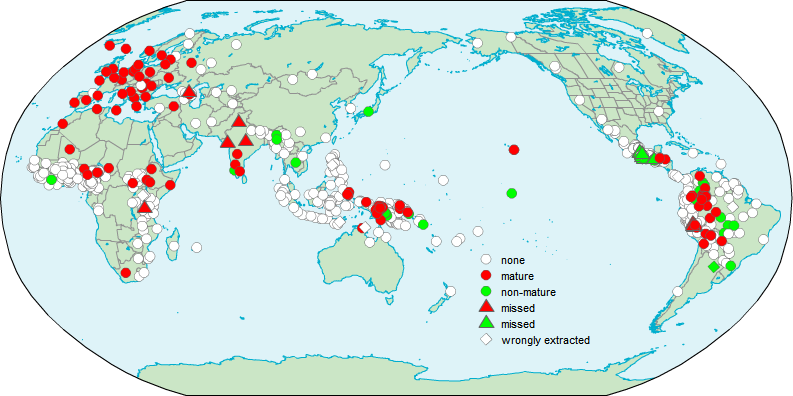
\includegraphics[width=\textwidth]{figures/12/12-fig1.png}
\end{minipage}\\
\begin{minipage}[t]{0.3\textwidth}
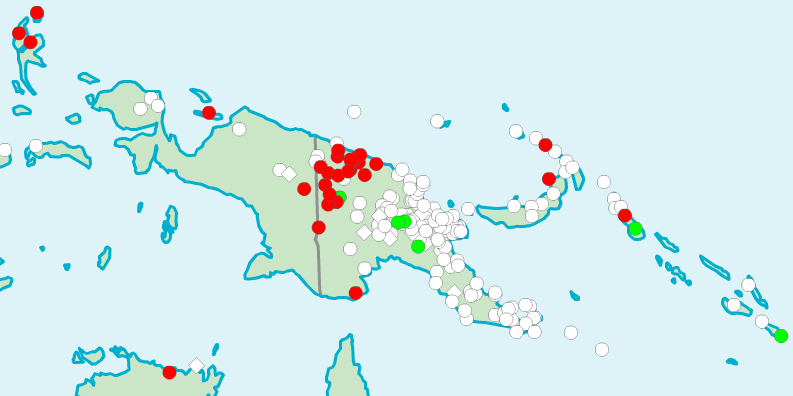
\includegraphics[width=\textwidth]{figures/12/12-fig1a.png}
\end{minipage}
\begin{minipage}[t]{0.3\textwidth}
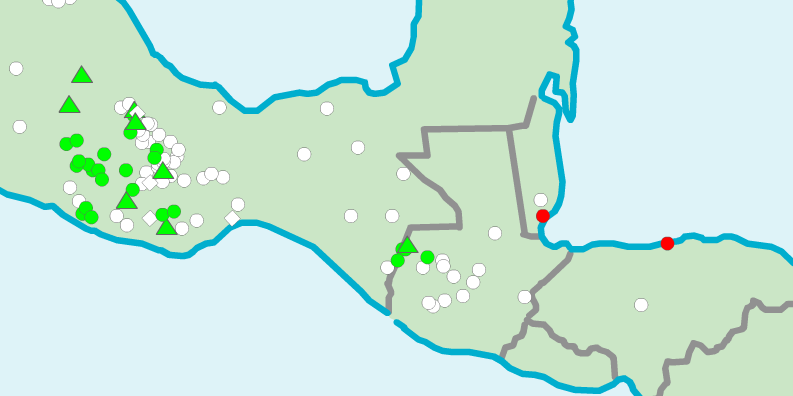
\includegraphics[width=\textwidth]{figures/12/12-fig1b.png}
\end{minipage}
\begin{minipage}[t]{0.3\textwidth}
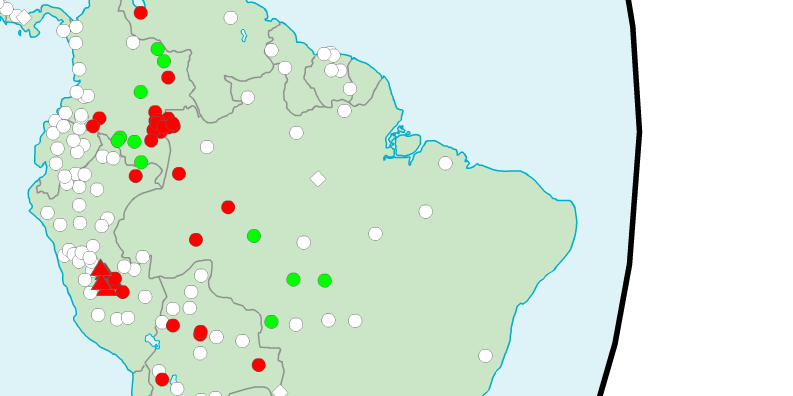
\includegraphics[width=\textwidth]{figures/12/12-fig1c.png}
\end{minipage}\\
{\small Map designed with the WALS Interactive Reference Tool by Hans-Jörg Bibiko.}
\caption{Languages of the sample with mature and non-mature feminine gender grams}
\label{fig:BW:1}
\end{figure}

Let us now discuss the languages listed in Table 5 one-by-one:

While English has a feminine marker for all relations \textendash{} \textit{she} for subject and \textit{her} for all other ones \textendash{} Belize Kriol English (at least the N.T.\ version) distinguishes feminine \textit{shee} only for S and A (subject); object \textit{ahn} and the possessor \textit{ih} do not distinguish gender. Even though there is only one form, there is different behavior across grammatical relations since the single feminine form does not occur as non-subject, where gender is neutralized in Belize Kriol English.

Agreement of possessors with head nouns is indicated by AGR in \tabref{tab:BW:5} and illustrated in (\ref{ex:BW:13}) for German and (\ref{ex:BW:14}) for Au. These examples show that gender indexation (boldface) and NP-internal gender agreement (arrow) can be expressed on the same word form.

\protectedex{%
\ea\label{ex:BW:13}
German (Indo-European; Mk.~3:31 ; Matth.~14:8)\\
\begin{xlist}
\ex
\gll \textbf{sein}-e	Mutter\\
{\textsc{poss.3sg.\textbf{m}-nom.sg.f}\textleftarrow}	Mutter(\textsc{f})[\textsc{nom}]\\
\glt ‘\textbf{his} mother’\\
\ex
\gll von	\textbf{ihr}-er	Mutter\\
from	{\textsc{poss.3sg.\textbf{f}-dat.sg.f}\textleftarrow}	mother(\textsc{f})[\textsc{dat}]\\
\glt ‘by \textbf{her} mother’\\
\end{xlist}
\z
}%

\ea\label{ex:BW:14}
Au (Toricelli; Mk.~3:31, Mk.~9:21, Matth.~14:11)\\
\begin{xlist}
\ex
\gll miye 	p-\textbf{ɨrak}\\
mother(\textsc{f})	{\textrightarrow\textsc{sg.f-poss.3sg.\textbf{m}}}\\
\glt ‘\textbf{his} mother’\\
\ex
\gll
haai 	k-\textbf{ɨrak}\\
father(\textsc{m})	{\textrightarrow\textsc{sg.m-poss.3sg.\textbf{m}}}\\
\glt ‘\textbf{his} father’\\
\ex
\gll miye 	p-\textbf{ɨre}\\
mother(\textsc{f})	{\textrightarrow\textsc{sg.f-poss.3sg.\textbf{f}}}\\
\glt ‘\textbf{her} mother’\\
\end{xlist}
\z

Welsh (\ref{ex:BW:15}) represents a special case in that anaphoric gender in possessive pronouns is marked only as a sandhi phenomenon spread to the following head noun. The third person singular masculine form \textit{ei} causes soft mutation (among other things \textit{m-}>\textit{f-}); the third person singular feminine form \textit{ei}, however, causes aspirate mutation (no change for \textit{m-}). This looks as if there was agreement into the wrong direction, but is simply a rather intricate case of anaphoric gender marking.

\ea\label{ex:BW:15}
Welsh (Indo-European; Matth.~14:8, Matth.~12:46)\\
\begin{xlist}
\ex
\gll \textbf{ei} 	\textbf{f}am\\
\textsc{poss.3sg}	\textsc{poss.3sg.\textbf{m}}:mother(\textsc{f})\\
\glt ‘\textbf{his} mother’\\
\ex
\gll \textbf{ei} 	\textbf{m}am\\
\textsc{poss.3sg}	\textsc{poss.3sg.\textbf{f}}:mother(\textsc{f})\\
\glt ‘\textbf{her} mother’\\
\end{xlist}
\z

Latin lacks gender distinctions in the dative and in the possessor (both non-reflexive \textit{eius} and reflexive \textit{su}-AGR). Latvian lacks a gender distinction for the direct object (\textit{viņu} \textsc{acc.sg.m/f}) and for reflexive possessors (\textit{sav}-AGR \textsc{rposs.m/f}). In the subject, gender in Latvian is indexed not only by the free pronoun, but sometimes also in participles (\textit{-usi} \textsc{ptcp.pst.act.nom.sg.f}). Northern Kurdish distinguishes gender in the oblique (\textit{wî} \textsc{m}, \textit{wê} \textsc{f}), which covers A (ergative), R and non-reflexive possessor, but not in the absolutive (\textit{ew} \textsc{m/f}) S and P relations. Hindi lacks gender in free pronouns, and in the perfective past, which I take here as the most representative form since it is used in narrative function, gender is marked on the verb (\textit{-ī} \textsc{f}) only in intransitive verbs and in some transitive verbs for the object. Ama (see also (\ref{ex:BW:3})) marks gender on the verb, but only for the absolutive, which, however, also covers the primary object (P and R): \textit{ko-so-ki} [see-\textsc{o.3sg.f-rem.pst}] ‘s/he saw her’ vs.\ \textit{ki-Ø-ki} [see-\textsc{o.3sg.m-rem.pst}] ‘s/he saw him’, \textit{i-so-ki} [say-\textsc{o.3sg.f-rem.pst}] ‘s/he said to her’ vs.\ \textit{i-mo-ki} [say-o.3sg.m%
\footnote{%
The masculine form is zero except for a few relics with \textit{-mo-} as in the verb ‘say’.
}%
\textsc{-rem.pst}] (\citealt{Arsjoe1999}).%
\footnote{%
Some predicates are especially salient in terms of frequency in the corpus with animate participants, these are notably ‘go/come/arrive’ for S, ‘see’ for P, and ‘say’ for R. However, the indexes listed in \tabref{tab:BW:2} are not always equivalent in translation; for instance, not in all languages ‘see’ is transitive.
}%

In all languages listed in \tabref{tab:BW:5}, anaphoric gender is well entrenched, which can be seen from the fact that its marker interacts in some way with grammatical relations, either by means of cumulation or neutralization. This situation is characteristic of mature gender grams where anaphoric gender has a long history. This is opposed to incipient gender marking where the gender gram is less complex and usually only has a single form irrespective of grammatical relation and where the use of the gram tends to be optional.

All examples in \tabref{tab:BW:5} have in common that anaphoric gender marking is pronominal (whether free or bound) and has variable formal expression across grammatical relations as opposed to the invariant anaphoric gender markers of nominal origin or supposedly nominal origin discussed in \sectref{sec:BW:3}. However, not all invariant anaphoric gender markers can be proven to have nominal origin. There are, for instance, two Tupian languages in the sample with invariant markers. \spterml{Kayabi} \textit{ẽẽ} \textsc{f} (male speaker) \textsc{m}, \textit{kyna} \textsc{f} (female speaker), \textsc{m} \textit{'ga} (male speaker), and \textit{kĩã} \textsc{m} (female speaker), distinguishing both speaker and referent gender. These markers also follow person names and animate nouns in anaphoric use. \spterml{Tenharim} has \textit{hẽa} \textsc{f} and \textit{'ga} \textsc{m} (singular and plural), which also occur as suffixes on referring person names and animate nouns. Like in other Tupian languages the pronominal prefixes on nouns and verbs do not distinguish gender in Kayabi (\citealt[27]{Dobson2005}) and Tenharim (\citealt[17]{Betts1981}). The lack of gender markers in most Tupian languages might suggest that anaphoric gender in Kayabi and Tenharim are innovations.

However, invariant marking does not always testify to recent origin of gender. \spterml{Malayalam} (Dravidian) has the constant pronominal stem \textit{avaḷ(-)} \textsc{3sg.f} and no bound pronouns. But Old Malayalam still had subject indexes on the verb (\textit{-ǟḷ} \textsc{3sg.f}) (\citealt[120]{Andronov1996}). Anaphoric gender marking was thus not invariant in Old Malayalam. While all Indo-European languages and all Creole languages with anaphoric gender in the sample have variant anaphoric gender marking, the artificial language \spterml{Esperanto} has invariant marking with the constant markers \textit{sxi(-)} \textsc{f} and \textit{li(-)} \textsc{m}.

Anaphoric gender can occasionally have quite unexpected sources. In \spterml{Yagua}, women who have borne children are referred to by dual forms (\citealt[42]{Payne1985}) \textendash{} \textsc{3du} \textit{naada-} (often realized as \textit{naan-}), \textit{naadá}, \textsc{2du} \textit{sáána-}, \textit{saadá}. Men, however, are referred to with singular bound pronouns: \textsc{3sg} \textit{sa-} [I], \textit{-níí} [II], \textsc{2sg} \textit{jiy-} [I], \textit{jíy} [II].%
\footnote{%
Set II forms are used for direct objects and some intransitive subjects.
} %
In the N.T.\ dual forms are used as a default for adult women for whom it is not specified in the text whether they have given birth to children. Even if this is lack of gender from the point of view of the system \textendash{} and Payne (\citealt*[42]{Payne1985}) says explicitly that Yagua lacks gender \textendash{} this is an anaphoric gender marking opposition from the point of view of language use. Anaphoric gender in Yagua hijacks another highly grammaticalized category, number. This is why the markers are mature even if they are presumably young as gender markers. Yagua is thus an example of a very specific origin of an anaphoric gender opposition which has a mature marker from the very beginning. However, since the origin of gender is often associated with case or number (\citealtv{Waelchlithisyeara}), the example of Yagua is perhaps less parochial than it seems at first glance.

To summarize: Even though there are a few exceptions, cumulation and/or neutralization testify to mature anaphoric gender marking whereas lack of cumulation and/or neutralization typically goes hand in hand with incipient gender marking. Since cumulation and neutralization can be considered to reflect an increase in complexity, this is evidence that complexity in anaphoric gender increases over time.

\section{Grammatical anaphors and incipient anaphoric gender markers}
\label{sec:BW:5}

\subsection{Introduction}
\label{sec:BW:5.1}

Third person pronouns (\textit{he/she}) and full NPs have very similar properties in anaphoric function. Notably, there is very little semantic difference between a gender marked anaphoric pronouns (\textit{he/she}) and a full definite NPs containing a light noun (a noun with a very general meaning, such as ‘man’, ‘woman’, ‘thing’). This contrasts with their very different form \textendash{} pronoun vs.\ noun \textendash{} which assigns them entirely different roles in the typology of referential devices. As mentioned above, \citet{Kibrik2011} makes a distinction between full referential devices (common nouns with or without modifiers, and person names) and reduced referential devices (pronouns and zero forms) and claims that it is universal: “The only truly universal opposition is that between full and reduced referential devices” (\citealt[42]{Kibrik2011}). Grammatical anaphors are intermediate referential devices in the sense that they are neither lexical nouns nor third person pronouns. However, the distinction is still clear-cut in the sense that grammatical anaphors are grammatical in the same way as personal pronouns and hence to be included when discussing gender grams. \citet[123--136]{Kibrik2011} discusses several of the grammatical anaphors considered here, such as Jacaltec classifiers and Japanese \textit{kare} ‘he’ and \textit{kanojo} ‘she’, under the heading “functional analogues” of personal pronouns.

Describing grammatical anaphors is essentially a synchronic aim. However, since grammaticalization tends to be unidirectional (\citealt{Haspelmath1999}) and intermediate forms do not seem to evolve from more grammaticalized pronominal anaphoric gender markers, there is automatically also a diachronic dimension. Put differently, forms intermediate between nouns and indexes also tend to be \spterm{incipient gender markers}. Intermediate forms (grammatical anaphors) keep from their lexical origin the property of distinguishing the basically lexical meanings ‘woman’ and ‘man’, but they are decategorialized from the lexical category of nouns. However, since the diachrony of grammatical anaphors often remains opaque, this is in some cases only a hypothesis. It is important to point out that incipient gender markers do not necessarily further grammaticalize to mature gender markers. It is very well possible that incipient gender markers can be lost or remain incipient. As discussed in \sectref{sec:BW:4}, mature gender markers can develop from other grammatical categories, such as number, case or person, and need not necessarily develop from incipient anaphoric gender markers.

Grammatical anaphors have both pronominal and nominal properties. Three different subtypes are discussed in this section as illustrated in \tabref{tab:BW:6}.

\begin{table}
\begin{tabularx}{\textwidth}{QQl}
\lsptoprule
Subtype	&	Example	&	Subsection	\\
\midrule
Non-compositional complex NP	&	Japanese \textit{kano(-)jo} *‘that(-)woman’	&	\sectref{sec:BW:5.2}	\\
Reduced nominal anaphor	&	Chalcatongo Mixtec \textit{-ña} (\textit{ñã’ã} ‘woman’)	&	\sectref{sec:BW:5.3}	\\
General noun	&	Northern Khmer \textit{niang} ‘girl; she’	&	\sectref{sec:BW:5.4}	\\
\lspbottomrule
\end{tabularx}
\caption{Three subtypes of grammatical anaphors}
\label{tab:BW:6}
\end{table}

Non-compositional complex NPs differ from the other types in that they are diachronically complex (more than one morpheme). Reduced nominal anaphors differ from the other two simplex types in that they diachronically reflect reduced nouns. General nouns have the form of a non-reduced noun, but they are so extended in use that they are semantically difficult to distinguish from pronouns. What makes them pronoun-like is not their form or word class, but the fact that their use is broader than in their lexical nominal use. Put differently, general nouns have specific meaning when used as nouns and more general meaning when used as grammatical anaphors.

Two further issues need to be specified. The first one is that not all instances of incipient anaphoric gender markers reflect genuine grammaticalization developments since linguistic gender categories can be subject to deliberate language planning. As there are sometimes attempts to eliminate anaphoric gender by language planning (for instance, in Swedish, a gender neutral form \textit{hen} has been suggested to replace \textit{han} ‘he’ and \textit{hon} ‘she’ and is now partly gaining ground especially in generic use; see \citealt[27]{Milles2011}), there have been attempts to implement gender distinctions in pronouns where there a none. A case in point is Uduk where the N.T.\ uses the noun \textit{(a)yim} [\textsc{class2}] ‘female friend’ for ‘she’ even though this noun does not have any anaphoric use in spoken Uduk (Don Killian, p.c.). Thus, Bible translation Uduk has a special pronominal noun whereas there are no indications of a grammaticalization of an anaphoric gender gram in spoken Uduk (for more information on gender in Uduk, see \citealtv{Killianthisyear}).

The second one is that the presence of a masculine grammatical anaphor does not entail the presence of a feminine form.%
\footnote{%
I do not know of any case of the contrary, a feminine grammatical anaphor without a corresponding masculine form.
} %
As other Mek languages, Yale (\ref{ex:BW:13}) has a masculine, but no feminine grammatical anaphor. Yale does not distinguish gender in third person pronouns (\textit{el} \textsc{3sg}), but has a special form bone glossed ‘this.man’ by \citet{Heeschen1992}, which does not contain the noun \textit{nimi} ‘man’, but rather looks like a demonstrative pronoun as it cumulates the expression of spatial deixis with its nominal meaning (\textit{ane} ‘this here’, \textit{ani} ‘that up there’, \textit{anu} ‘that down there’, \textit{bini} ‘that man up there’, \textit{bunu} ‘that man down there’; \citealt[15]{Heeschen1992}). All three devices, demonstrative NP, grammatical anaphor and personal pronoun, occur in example (\ref{ex:BW:16}) and are summarized in \tabref{tab:BW:7}.

\ea\label{ex:BW:16}
Yale (Mek, Trans-New Guinea phylum; \citealt[29]{Heeschen1992})\\
\gll \textbf{Nimi}	\textbf{ane}	dinge,	\textbf{bone}	dinge	dane,	\textbf{el}-di	kwaneng	wa-m-la=ba, na	do-do	de-n.\\
man	this	property,	this.man	property	\textsc{dem:pl}	\textsc{3sg-gen}	sweet.potato	be-\textsc{prf-prs.3sg}=\textsc{connect} \textsc{1sg}	take-\textsc{cvb}	eat\textsc{[pfv].prs.1sg}\\
\glt ‘I have taken and eaten (earlier today) this man’s sweet potatoes.’\\
\z

While the etymology of \textit{bone} ‘this.man’ is opaque, there is a second grammatical anaphor in Yale which obviously derives from a full NP: \textit{mene} ‘this.child’ (\textit{mini} ‘that child up there’, \textit{munu} ‘that child down there’ < \textit{me ane/ani/anu}).

\begin{table}
\begin{tabularx}{\textwidth}{lQQ}
\lsptoprule
\scshape 3sg	&	Grammatical anaphors	&	N \scshape dem	\\
\midrule
	&	\textit{bone} ‘this.man’	&	\textit{nimi ane/ene} ‘this man’	\\
\textit{el} ‘she/he’	&	—	&	\textit{kel ane/ene} ‘this woman’	\\
	&	\textit{mene} ‘this.child’	&	\textit{me ane/ene} ‘this child’	\\
\lspbottomrule
\end{tabularx}
\caption{Yale third person pronouns, grammatical anaphors and demonstrative NPs}
\label{tab:BW:7}
\end{table}

This section does not discuss all languages in the sample where gender has emerged recently. Due to genealogical considerations, in some languages feminine gender must have emerged recently (all related languages lack feminine; this holds, e.g., for Northern Wè within Niger-Congo; \citealt{Paradis1983}), but it is not possible to trace a non-pronominal origin of gender markers.

It should be also stressed that automatic extraction of anaphoric gender (\sectref{sec:BW:3}) has been the dominant heuristic in identifying the relevant set of languages. Many languages discussed here are not traditionally considered gender languages and when I obtained forms in the automatic extraction I first thought that there must be some mistake in the algorithm.%
\footnote{%
Since many languages also have third person singular forms not distinguishing gender they are not usually captured in Siewierska’s (\citealt*{Siewierska2005}) typology (except Japanese where the third person singular pronoun is zero anaphor).
}%

Some of the forms to be discussed in this section figure prominently in the literature on classifiers, especially \spterm{noun classifiers}. This is no surprise since anaphoric use is a well-recognized function of noun classifiers in some languages. According to \citet[87]{Aikhenvald2000} “noun classifiers are typically used with anaphoric function”. Aikhenvald discusses especially Mayan languages of the Kanjobalan branch (Jacaltec and Akateko) and some Australian languages (notably Yidiny). It is thus not unexpected that some noun classifier languages are found to exhibit anaphoric gender which does not presuppose agreement as definitional property.

The literature on noun classifiers has in common with the literature on gender that it considers anaphoric use to be secondary. Noun classifiers as grammatical markers co-occurring with nouns in the same NP are not the topic of this paper, and in the same way as anaphoric gender can be considered without making reference to the notion of agreement, it can also be considered without making reference to the notion of noun classifiers.


\subsection{Non-compositional complex NPs}
\label{sec:BW:5.2}

Non-compositional complex NPs have similar uses as expressions for ‘that woman/man’, and sometimes they are entirely opaque, as the example from Kiribati illustrated in \sectref{sec:BW:1}. However, non-compositional complex NPs are not usually condensed forms of ‘that woman/man’; rather they contain other nouns that have been generalized to general meanings of feminine or masculine, such as ‘mother’ or ‘elder sister’ or ‘body’ or they contain obsolete or irregular forms of demonstrative pronouns.

English has no anaphoric non-compositional NPs, but a related phenomenon is indefinite pronouns originating from NPs, such as \textit{somebody}. \textit{Somebody} contains the noun \textit{body}, but does not have the meaning that the noun \textit{body} has. For a typology of indefinite pronouns, see \citet{Haspelmath1997}. In the languages of the sample, non-compositional complex NPs are attested in Kiribati (Austronesian), Japanese (isolate), Kannada (Dravidian), Zome (Sino-Tibetan), Golin and Chuave (Chimbu, Trans-New Guinea phylum). Anaphoric gender markers in some South American languages with noun classifiers, notably Nambikuara and in Guahiban and Witotoan languages, are highly reminiscent of non-compositional complex NPs and can perhaps be interpreted as more advanced stages of grammaticalization. \tabref{tab:BW:8} summarizes the forms of the languages discussed in this section.

\begin{table}
\begin{tabularx}{\textwidth}{Q>{\itshape}X>{\itshape}X>{\itshape}X>{\itshape}X}
\lsptoprule
& \normalfont	Index (3sg general)	&	\normalfont Grammatical anaphor	&	\normalfont NP ‘that woman’	&	\normalfont ‘woman’	\\
\midrule
Japanese	&	\normalfont zero anaphor	&	kanojo	&	sono onna	&	onna	\\
Kannada	&	avaḷu {\normalfont (\scshape f)}, {\normalfont V}-aḷu {\normalfont (\scshape f)}	&	āke \normalfont (honorif.)	&	ā strīyu	&	strīyu	\\
Zome	&	amah	&	tuanu	&	tua numei	&	numei	\\
Kiribati	&	ngaia, e	&	neierei	&	te aiine aarei	&	aiine	\\
Golin	&	{\normalfont V}-m, {\normalfont V}-ngw	&	abalini	&	abal i	&	abal	\\
Chuave	&	{\normalfont V}-m, {\normalfont V}-ngu	&	oparomi	&	opai, 	&	opai	\\
S.~Nambikuara	&	te²na², {\normalfont zero}, {\normalfont V}-la¹	&	ta¹ka³lx(ai²n)a²	&	txu¹h(a³ka³lx)ai²na²	&	txu¹ha²	\\
Cuiba	&	$-$	&	barapowa	&	barapo petsiriwa/ yabʉyo	&	yabʉyo, petsiriwa	\\
Guayabero	&	$-$ 	&	-ow, hapow	&	ampow pawis	&	pawis	\\
Huitoto Murui	&	ie	&	naiñaiño	&	naie rɨño	&	rɨño	\\
Huitoto Minica	&	ie	&	afengo	&	afe rɨngo	&	rɨngo	\\
Bora	&	(i-)	&	diílle, -lle	&	áalle	&	walle	\\
\lspbottomrule
\end{tabularx}
\caption{Languages with non-compositional complex NPs for female reference}
\label{tab:BW:8}
\end{table}

\spterml{Japanese} \textit{kanojo} ‘she’ means originally ‘that woman’, but it is not a reduced form of \textit{sono onna} [that woman] ‘that woman’. \textit{Kano} is originally the attributive form of a distal demonstrative (free form \textit{kare}) that has come out of use except in a few fixed archaic expressions such as \textit{kare kore} ‘that and this’. \textit{Jo} is the Sino-Japanese expression for ‘woman’ (\citealt[141]{Ishiyama2008}). \textit{Kanojo} and its masculine counterpart \textit{kare} ‘he’ (originally ‘that’) were established in the Meiji period (1868--1912) in the literary movement \textit{genbun-itchi} (unification of written and spoken language) where translations from European languages played an important role (\citealt[139]{Ishiyama2008}). There is some element of deliberate manipulation in this grammaticalization process and there is no reduction or erosion contributing to the grammaticalization of \textit{kanojo} ‘she’. The reason why \textit{kanojo} cannot be analyzed as a compositional NP anymore is that the demonstrative \textit{kano} has disappeared. Although \textit{kanojo} usually is translated with ‘she’ it could also still be translated as ‘that woman’. In the N.T.\ \textit{kanojo} competes in the anaphoric domain with \textit{onna} ‘woman’ and \textit{sono onna} ‘that woman’ (\textit{suruto onna ha itsut-ta} [and woman \textsc{top} say-\textsc{pst}] ‘So she said’; Matth.~15:27). \textit{Kanojo} and \textit{kare} cannot be compared to \textit{she} and \textit{he} in terms of text frequency (\citealt[36]{Ishiyama2008}). Japanese prefers zero anaphor as reduced referential device (\citealt[44]{Kibrik2011}). \textit{Kanojo} also has some rather nominal uses: \textit{kanojo wa?} [she \textsc{top}] ‘Do you have a girlfriend?’ (\citealt[232]{Ishiyama2008}). It can also be used as a term for address (\citealt[232]{Ishiyama2008}) which further shows that it is not a canonical third person pronoun.

\spterml{Kannada} (Dravidian) has so called honorific pronouns \textit{āke} ‘that woman, she’, \textit{īke} ‘this woman’, which have developed from the demonstratives \textit{ā} ‘that’, \textit{ī} ‘this’ and \textit{akka} ‘elder sister’. The second component in \textit{ātanu} ‘that man, he’, \textit{ītanu} ‘this man’ (honorific) is of Sanskrit origin: \textit{dēha-} ‘person, body’. Similar forms are found in Telugu (\citealt[171]{Andronov2003}). Kannada and Telugu are the only languages I am aware of which have both gender-distinguishing third person pronouns (Kannada \textit{avaḷu} ‘she’, \textit{avanu} ‘he’) and grammatical anaphors.

\spterml{Zome} (Sino-Tibetan) \textit{nu} and \textit{pa} mean ‘mother’ and ‘father’ when possessed (\textit{ka/na/a nu} [\textsc{1sg/2sg/3sg} mother]), but with the demonstratives \textit{tua} ‘that’ and \textit{hih} ‘this’ they are non-compositional complex NPs: \textit{tuanu} ‘that woman, she’, \textit{hih nu} ‘this woman, she’. The corresponding nouns are \textit{numei} ‘woman’ and \textit{mi} ‘man’. Rather than just pronouns and NPs there are three sets of forms in Zome: \textit{ama(h)} ‘he/she’, \textit{tuanu} ‘she, that woman’, and \textit{tua numei} ‘that woman’. It might be argued that \textit{tuanu} ‘that woman, she’ is not sufficiently opaque to qualify as a non-compositional complex NP and is not much different from cases such as South Tairora \textit{nraakyeva} [\textit{nraakye-va} ‘woman-\textsc{dem}'] that have been removed as errors (see \sectref{sec:BW:3.4}(a)). Indeed, no form is extracted for Zome if the form is spaced \textit{tua nu}, where \textit{nu} ‘mother’ is removed by the ‘mother’ filter. However, Zome is different from South Tairora in that the demonstrative is written without space only in few forms where it is semantically non-compositional, it is not generally an affix. Looking more closely for non-univerbated collocations of ‘that mother’ in the search domain in other Sino-Tibetan languages did not yield any further cases like Zome \textit{hih nu} ‘this woman, she’, which suggests that Zome is different from other Sino-Tibetan languages in the sample.

In the variety of \spterml{Golin} (Trans New Guinea, Chimbu) documented by \citet[55]{Bunn1974}) which is the same as in the N.T., the pronouns for third person plural \textit{abalíni} ‘she’ < \textit{abál inín} [woman \textsc{refl}] and \textit{yalíni} ‘he’ < \textit{yál inín} [man \textsc{refl}],%
\footnote{%
The N.T. also has a few occurrences of \textit{ibalini} (\textit{ibal} ‘people’).

The documentation of Golin by \citet{Evans2005} has \textit{yal (i) inin} ‘he’ [man \textsc{(top) refl}] only twice and in both cases \textit{inin} can be interpreted reflexively.
} %
are not reflexive although they seem to contain reflexive markers. The variety documented by \citet{Evans2005} does not seem to have the same forms, but even this variety uses almost consistently NPs containing \textit{abal} ‘woman’ or \textit{gi} ‘girl’ and \textit{yal} ‘man’ wherever the English translation has ‘she’ or ‘he’ as in (\ref{ex:BW:17}) while in few cases where the reference is repeated within the same sentence there is only a bound affix for third person which does not distinguish gender.

\ea\label{ex:BW:17}
Golin (\citealt[35]{Lee2005})\\
\gll abal 	i 	takal 	no-m \\
woman	\textsc{top} 	what 	eat-3\\
\glt ‘What did she eat?’\\
\z

In the closely related language Chuave \textit{opai} ‘woman’ and \textit{yai} ‘man’ are opposed to \textit{opa-rom-i} ‘woman-?-\textsc{dist} and \textit{ya-rom-i/day} ‘man-?-\textsc{dist/prox}’ (\citealt{Thurman1987}) where the element \textit{-rom-}, misleadingly glossed ‘this’ by Thurman, only occurs in these two non-compositional anaphoric forms.

In \spterml{Southern Nambikuara} (Nambiquaran) \textit{txu¹ha²} ‘woman’ is opposed to \textit{ta¹ka³lxai²na²} ‘the woman, she’ (\textit{in³txa²} ‘man’ vs.\ \textit{jah¹lai²na²} ‘the man, he’). \textit{Ta¹ka³lxai²na²} and \textit{jah¹lai²na²} are listed as third singular feminine free pronouns by \citet[283]{Lowe1999} even though they contain the demonstrative nominal ending \textit{-ai²na²} and the base can take many other nominal endings including demonstrative emphatic \mbox{\textit{-ai²li²}} and indefinite \textit{-su²} (\textit{ta¹ka³lxu²su²} once in the N.T.\ for ‘a woman’).%
\footnote{%
Note, however, that even the free forms for first and second person have the demonstrative and emphatic noun suffixes \textit{txai²na²/txai²li²} ‘I’, \textit{wxãi²na²/wxãi²li²} ‘you’, but they do not take the definite and the indefinite endings.
} %
\citet[71]{Kroeker2001} gives instead the forms with definite suffix (\textit{-a²}) as third person forms (\textit{ta¹ka³lxa²} and \textit{jah¹la²}). There is also a third person form \textit{te²na²} not distinguishing gender, which is used mostly in generic contexts where gender is not specified. Nambikuara has a large set of noun classifiers including \textit{-a³ka³lx(i³)} feminine and \textit{-(j)ah¹lo²} masculine which are always followed by nominal endings. These classifiers are placed at the end of NPs following adjectives and relative clauses. Thus, example (\ref{ex:BW:18}) is one noun phrase. I interpret \textit{Ta¹ka³lx(ai²n)a²} and \textit{jah¹l(ai²n)a²} as non-compositional complex NPs.

\ea\label{ex:BW:18}
Southern Nambikuara (Rev.~17:18)\\
\gll txu¹ha²	ta¹ka³lx-a²	ĩ²-in¹-ta³ka³lx-ai²na²	\\
woman	woman[\textsc{ana}]-\textsc{def}	see-\textsc{2sg-f-dem}\\
\glt ‘the woman whom thou sawest’\\
\z

In Guahiban and Witotoan languages feminine anaphoric and masculine forms consist of demonstratives with classifier suffixes which can perhaps be considered opaque grammaticalized forms of non-compositional complex NPs.

Guahiban languages use demonstratives with classifier suffixes as special anaphoric forms. Guayabero differs from Cuiba and Guahibo in that the forms have become bound indexes on verbs, which suggests a higher degree of grammaticalization. \spterml{Cuiba} (Guahiban) has the demonstratives \textit{ba(ra)po-wa}, \textit{po-wa} [this-\textsc{f}, that-\textsc{f}] and \textit{ba(ra)po-n}, \textit{po-n} [this-M, that-M]. \citet[237]{Machal2000} lists the proximal <\textit{bajapowa/bajaponü}> as personal pronouns, \citet[589]{Merchan2000} the distal \textit{powa/pon}; neither source mentions the forms \textit{barapowa/barapon}.
In the N.T.\ mainly the forms \textit{ba(ra)powa/ba(ra)pon} are used anaphorically \textendash{} both longer and shorter forms very much in similar contexts \textendash{} often also preposed to person names in anaphoric use. \textit{Powa/pon} are mostly used NP-internally as a relative clause introducer. The suffixes \textit{-wa} F and \textit{-n} M make part of a larger set of classifier suffixes. Merchán (2000: 589) lists eight other inanimate suffixes, which do not seem to occur with demonstrative stems, however. Attributive demonstratives usually lack classifier markers. For the closely related language \spterml{Guahibo}, de Kondo (1985, 1: 15) gives \textit{pów\underline{a}}
F and \textit{pón\underline{ë}} M as personal pronouns (which are, however, used only in relative function in the N.T.\ and rare) and the forms with proximal circumfix \textit{m\underline{a}-je} and distal prefix \textit{baja-} as demonstratives (de Kondo 1985, 2: 49). In the N.T.\ \textit{barapova} is the dominant feminine anaphoric form; \textit{mapovaje} is mainly used for ‘this woman’, a combination of demonstrative and \textit{petiriva} woman (\textit{bajarapova petiriva}) is attested only once; for definite uses of ‘woman’ the demonstrative with the feminine classifier suffix is preferred in proximal or distal form. \spterml{Guayabero}, a third Guahiban language, is different in that F \textit{-(p)ow} and M \textit{-(p)on} are used as bound indexes on verbs if there is no NP subject (they are two of at least nine third person markers, including various diminutive and neuter forms, see Keels 1985: 79, 86) and have become the major anaphor in the subject relation rather than the demonstratives \textit{japow} and \textit{japon}. According to Keels (1985: 79), subject and object indices can be combined on the same verb, but in the N.T.\ the object is usually expressed by the full pronoun \textit{japow/japon}. The tendency to reduce subject markers more often than object markers can be seen as a first trait of maturity in Guayabero anaphoric indexes.

The special anaphoric form in \spterml{Huitoto Minica} (Witotoan) \textit{afengo} ‘she, that woman’ (masculine \textit{afemɨe}) consists of the demonstrative \textit{afe} ‘that’ and the feminine noun classifier \textit{-ngo} (masculine \textit{-mie}) and is opposed to the noun \textit{rɨngo} ‘woman’ (\textit{ɨima} ‘man’) (\citealt{Minor1982}). The demonstrative can also combine with the noun: \textit{afe rɨngo} ‘that woman’, \textit{bie ringo} ‘this woman’. The numeral for ‘one’ can combine both with the noun \textit{daa ringo} ‘a woman’ and the classifier \textit{daa-ngo} ‘a woman’ (rare). There is also a third person singular pronoun \textit{ie} not distinguishing gender which is predominantly used in possessive function. \spterml{Huitoto Murui} is structurally very similar, except that the feminine classifier has various forms (\textit{-ño}, \textit{-ñaìño})
and is freer in combining with different pronominal stems (\textit{naì-ñaìño} \textsc{dem.dist-f}, \textit{baì-ñaìño} \textsc{dem.vis-f}, \textit{bi-ñaìño} \textsc{dem.prox-f}, \textit{i-ñaìño} \textsc{3sg-f}). However \textit{i-ñaìño} \textsc{3sg-f} is rare and never used as a pronominal form (it is rather a free form of the classifier suffix). The most dominant anaphoric form is the distal \textit{naìñaìño} ‘she; that/the woman’. It is a matter of debate how closely related Bora and Huitoto are, but as far as the domain discussed here is concerned, the structural parallels are very strong. The major difference is that the Bora classifiers are not restricted to nouns and nominalizations but have extended to indexation on verbs, which is why \spterml{Bora} \textit{-lle} ‘\textsc{f}’ and \spterml{Muinane} \textit{-go} ‘\textsc{f}’ are much more frequent than Huitoto Minica \textit{-ngo}. A special property of the Bora text is that the noun for ‘woman’, \textit{walle}, is very rare in the N.T.; it is used almost exclusively in generic contexts. Almost the whole range of the nominal domain is covered by the classifier suffix \textit{-lle}. With numerals, the classifier is used: \textit{tsáápille} ‘one/a woman’. The possessive prefix for third person \textit{i-} does not distinguish gender.

Non-compositional complex NPs tend not to be genealogically pervasive. They pop up occasionally in most different language families, except in Guahiban and Witotoan where we also encounter the most mature exemplars. It can be assumed that non-compositional complex NPs originate from transparent complex NPs when one of their parts becomes opaque or as they acquire a non-compositional meaning. However, the nominal origin is a hypothesis as far as Kiribati and the South American languages are concerned, where the etymology of the forms cannot be traced.


\subsection{Reduced nominal anaphors}
\label{sec:BW:5.3}

While the non-compositional complex NPs discussed in \sectref{sec:BW:5.2} are found in a wide range of language families, the reduced nominal anaphors in the sample all come from Mesoamerica and almost exclusively from one family, Otomanguean. \tabref{tab:BW:9} lists examples from six Otomanguean examples, where reduced nominal anaphors occur in subject and reflexive possessor roles.

\begin{table}
\begin{tabular}{l>{\setlength{\tabcolsep}{2pt}}l}
\lsptoprule
Tlalcoyalco Popoloca	& \multirow{2}{*}{
                        \begin{tabular}{*{8}{l}}
                        \itshape co & \itshape jehe &\itshape  xan &\itshape  joanjo &\itshape \bfseries xan &\itshape  ngain &\itshape  janné &\itshape  \bfseries xan\\
                        and& 3& child& gave&\bfseries child[\textsc{ana}]& give& mother& \bfseries child[\textsc{ana}]
                        \end{tabular}
                        }\\
\\
\padding
San Miguel Mixtec	    &	\multirow{2}{*}{
                        \begin{tabular}{*{6}{l}}
                        \itshape te &\itshape máá‑\textbf{i}, &\itshape ni̱ &\itshape jancha̱ka‑\textbf{i} &\itshape nuu̱ &\itshape náa̱‑\textbf{i}	\\
                        and &self-\textbf{\textsc{young}} &\textsc{compl} &gave-\textbf{\textsc{young}} &to &mother-\textbf{\textsc{young}}	\\
                        \end{tabular}
                        }\\
\\
\padding
Tepeuxila Cuicatec	 &	\multirow{2}{*}{
                        \begin{tabular}{*{8}{l}}
                        \itshape ní &\itshape \textbf{táⁿ'ā} &\itshape miiⁿ &\itshape ní &\itshape ca'a &\itshape \textbf{tá} &\itshape chɛɛcu &\itshape \textbf{tá}	\\
                        and &\textbf{woman.\textsc{f}} &there/\textsc{def} &? &\textsc{compl}:give:3 &\textbf{\textsc{f}} &mother &\textbf{\textsc{f}}	\\
                        \end{tabular}
                        }\\
\\
\padding
San Martín Itunyoso Triqui	&	\multirow{2}{*}{
                              \begin{tabular}{*{6}{l}}
                              \itshape ni̱ &\itshape naga'ui' &\itshape \textbf{ún'} &\itshape ra'a &\itshape nni &\itshape \textbf{ún'}	\\
                              and &gave &\textbf{\textsc{f}} &to &mother &\textbf{\textsc{f}}	\\
                              \end{tabular}
                              }\\
\\
\padding
Chiquihuitlan Mazatec	&	\multirow{2}{*}{
                        \begin{tabular}{*{5}{l}}
                        \itshape ca-sua &\itshape \textbf{na} &\itshape naa &\itshape rë &\itshape \textbf{na}	\\
                        \textsc{compl}-give &\textbf{\textsc{f}} &mother &\textsc{poss} &\textbf{\textsc{f}}	\\
                        \end{tabular}
                        }\\
\\
\padding
Amatlan Zapotec	&	      \multirow{2}{*}{
                        \begin{tabular}{*{7}{l}}
                        \itshape nu &\itshape lee &\itshape \textbf{me} &\itshape m-zaaya &\itshape lo &\itshape xnaa &\itshape \textbf{me}	\\
                        and &\textsc{foc} &\textbf{\textsc{f}} &\textsc{compl}-give &to &mother &\textbf{\textsc{f}}	\\
                        \end{tabular}
                        }\\
\\
\lspbottomrule
\end{tabular}
\caption{V-subject and N-reflexive possessor in ‘and she (=the girl) brought it to her mother’ (Matth.~14:11) in selected Otomanguean languages with anaphoric gender}
\label{tab:BW:9}
\end{table}


Reduced nominal anaphors in Otomanguean are both more grammaticalized and less grammaticalized than non-compositional complex NPs discussed in \sectref{sec:BW:5.2}. They are rather highly grammaticalized in that they quickly increase in token frequency as they extend to all grammatical relations including reflexive possessors. However, they tend to remain more restricted in use semantically. There can be separate forms for young humans, as in San Miguel Mixtec, and often there are separate forms for human respect and for deities.

In some languages the nominal origin of the reduced forms can clearly be traced. This is most obvious in Tlacoyalco Popoloca (\citealt{Stark2011}). Although Tlacoyalco Popoloca has a third person pronoun \textit{je\textquotesingle e} not distinguishing gender there is a large number of short forms of nouns with anaphoric use (termed “short pronouns” in \citealt[3]{Stark2011}). The most common include \textit{xii} ‘man[\textsc{sg}]’ (anaphoric \textit{xa}) and \textit{nchrii} ‘woman[\textsc{sg}]’ (anaphoric \textit{nchra}). Example (\ref{ex:BW:19}) illustrates a plain noun \textit{janna\textquotesingle a} ‘mother’ and its corresponding anaphoric form \textit{jan}:

\protectedex{%
\ea\label{ex:BW:19}
Tlacoyalco Popoloca (\citealt[4]{Stark2011})\\
\gll Naa	\textbf{janna\textquotesingle a}	jian	anseen	\textbf{jan}	ixin	rinao	\textbf{jan}	kain	xe\textquotesingle en	\textbf{jan}.\\
one	mother	fine	heart	mother[\textsc{ana}]	because	loves	mother[ANA]	all	children	mother[\textsc{ana}]\\
\glt ‘A mother has a good heart because she loves all her children.’ \\
\z
}%

Some condensed anaphoric NPs are reminiscent of noun classifiers (“pronouns that echo a prefix”; \citealt[4]{Stark2011}) and some uses are compatible with a noun class with agreement interpretation as when animals take the pronoun \textit{ba}. However, anaphoric noun formation is productive and applies even to Spanish loanwords (\textit{guitaarra}, anaphoric \textit{guitarra}).

Tlacoyalco Popoloca \textit{nchra} ‘woman[\textsc{ana}]’ is so specific in its meaning that it can hardly be considered a grammaticalized feminine gram. It has the distribution of a word for ‘woman’, and other female nouns have other anaphoric forms.

All \spterml{Mixtec} languages have clitic anaphoric gender markers usually following their head (following a verb for subject and object, following a relational noun for oblique and following a noun for possessor) which mostly have the phonological structure CV (see \citealt{Macri1983} for a survey of several Mixtec languages) and are much more strongly grammaticalized than Popoloca anaphoric nouns. Unlike first and second person, there are no full free forms for third person clitics, or rather the corresponding full free forms are nouns. \spterml{Chalcatongo Mixtec} (\citealt[139]{Macaulay1996}) has the following six sets (in parentheses the nouns corresponding to the reduced nominal anaphors): masculine \textit{-ðe} (\textit{čàà} ‘man’), feminine \textit{-ña} (\textit{ñã’ã} ‘woman’), polite, older \textit{-to} (\textit{to’ò} ‘older person’), supernatural \textit{-ža} (\textit{í’a}, \textit{íža} ‘god’), \textit{-tɨ} animal, and \textit{-ži} (no related noun, \textit{žii} is ‘male’). The clitics are usually not tenacious (i.e., they are dropped if there is an explicit NP), unless the NP preposed to the verb is a topic (\citealt[140]{Macaulay1996}). A way to supplete the missing full forms needed for contrastive purposes is to add the clitic to the emphatic form \textit{máá} ‘self’ (\citealt[106]{Macaulay1996}, see also \tabref{tab:BW:4} above). The meaning of Mixtec genders is much more general than those of Tlacoyalco Popoloca genders. But ‘girl, young women’ is often covered by the child gender in many Mixtec languages (see \tabref{tab:BW:9} for an example from San Miguel Mixtec). In \spterml{Coatzospan Mixtec}, feminine gender is of limited use since there is a general adult respect human gender \textit{ña} that does not distinguish men and women. “[T]he use of a specifically masculine or feminine noun or pronoun to refer to an adult is usually considered disrespectful” (\citealt[406]{Small1990}).

Reduced nominal anaphors or forms reminiscent of reduced nominal anaphors can also be found in Cuicatec (\citealt{Bradley1991}), in Chiquihuitlan Mazatec (\citealt{Capen1996}; but not in three other Mazatec languages included in the sample), and in Triqui (see \tabref{tab:BW:9}).

Most Zapotec languages have some forms that are intermediate between nouns and third person pronouns. Feminine is not always a salient category though, because many Zapotec languages have a special respectful form used for both genders, especially for women by men speaking. In \spterml{Texmelucan Zapotec} respect is used for deity, respect human in women’s speech and respect feminine in men’s speech (\citealt[290]{Speck1972}). Texmelucan Zapotec has masculine (\textit{yu}, \textit{-y}), feminine (\textit{fiñ}, \textit{ñi}, \textit{-ñ}), respect (\textit{mi}, \textit{-m}), animal (\textit{ma}, \textit{bañ}) and neuter (\textit{ñi}, \textit{-ñ}), which occur both in fuller and more reduced forms. As shown in (\ref{ex:BW:20}), masculine and feminine can be modified by adjectives, numerals, and demonstratives, which makes them look rather like nouns, but they can even be reduced subject indexes on verbs.

\ea\label{ex:BW:20}
Texmelucan Zapotec (\citealt[32]{Speck1972})\\
\gll Benu	sac	\uline{\textbf{fiñ}	feñ}	nu	gusht	ni	\textbf{yu}	feñ	ze´	lugaar	ze´	nu	cyiiñ	\textbf{yu}, \uline{\textbf{yu}	ze´}	neñ	\textbf{yu}	nu	zu	\uline{tub	\textbf{ñi}}	ca	zi´l	na 	tub	ranch	nu	zet, ze´	a´	yu´	lo	nap	\textbf{yu-ñ},	orze´	uz	\textbf{yu}	gzuu	nez	\textbf{yu}	i´ñ	\textbf{yu} \uline{\textbf{yu}	feñ}	ze´	nu	cha-\textbf{y}	cha	gwii-\textbf{y}	\uline{\textbf{fiñ}	mñaa	ze´} ben	a	gyet	lagy	\textbf{yu-ñ}.\\
if	not.be	\uline{\textbf{\textsc{3f}}	young}	\textsc{comp}	please	\textsc{pp}	\textbf{\textsc{3m}}	young	that	place	that	\textsc{comp}	\textsc{pot}:live	\textbf{\textsc{3m}} \uline{\textbf{\textsc{3m}}	that}	hear	\textbf{\textsc{3m}}	\textsc{comp}	\textsc{pot}:stand	\uline{one	\textbf{\textsc{3f}}}	where 	only 	be 	one	ranch	\textsc{comp}	far but	\textsc{neg}	\textsc{prog}.be.in	face	good	\textbf{\textsc{3m-3f}}	then	father 	\textbf{\textsc{3m}} 	\textsc{pot:caus}:stand	trail	\textbf{\textsc{3m}}	child	\textbf{\textsc{3m}} \uline{\textbf{\textsc{3m}}	young}	that	\textsc{comp}	\textsc{pot}:go-\textbf{\textsc{3m}} 	\textsc{pot}:go	\textsc{pot}:see-\textbf{\textsc{3m}}	\uline{\textbf{\textsc{3f}}	woman 	that} if	\textsc{q}	\textsc{pot}:descend 	liver	\textbf{\textsc{3m-3f}}\\
\glt ‘If there are no young women who appeal to the young man at the place where he lives, but if he hears that there is one at some ranch or another that is far away, but if he doesn’t know her well, his father will send his child, the young man, to go see if he likes her or not.’\\
\z

For \spterml{Mixtepec Zapotec}, \citet[11]{Hunnn.d.} list fourteen categories of third person pronouns, twelve of which refer to persons and only one of which is a reduced form (C\textit{-á}, V\textit{-w} inanimate). Their use depends on the speaker as is quite common across Zapotec: e.g., \textit{nîip}, \textit{nîib} is used by men for a young man and by women for a man of their age or younger. Several categories refer to men and women of lesser respect. \textit{Zhó} <zho> ‘person of minor respect, group of people’ is used, for instance, in the N.T.\ for the Samaritan (Lk.~10:33). Shifting use depending on speaker attitude is not easily understandable in terms of noun classes, but well in-line with the idea of anaphoric gender.

Gender is more strongly grammaticalized in \textbf{Southern Rincón Zapotec}, where the familiar forms lack a gender opposition and respectful forms distinguish masculine and feminine (\citealt[363]{Earl2006}). While the feminine consistently has the form \textit{-nu} (free form \textit{lë-nu}), the masculine form varies (free form \textit{lë-\textquotesingle}): \textit{blé\textquotesingle i-\textbf{në\textquotesingle}=nu} [\textsc{comp}.saw-\textsc{3sg.\textbf{m}.resp=3sg.f.resp}] ‘he saw her’, \textit{blé\textquotesingle i-nu=\textbf{në\textquotesingle}} [\textsc{compl}.see-\textsc{3sg.f.resp=3sg.\textbf{m}.resp}] ‘she see him’, \textit{cati\textquotesingle\ blé\textquotesingle i-\textbf{në\textquotesingle\ lë\textquotesingle}} [when \textsc{compl}.see-\textsc{3sg.\textbf{m}.resp} \textsc{3sg.\textbf{m}.resp}] ‘when he saw him’, \textit{rë-\textbf{\textquotesingle}‑nu} [\textsc{cont}.say-\textsc{3sg.\textbf{m}.resp-3sg.f.resp}] ‘he said to her’. The allomorphs cannot be clearly ascribed to different grammatical relations, however: \textit{-(ë)\textquotesingle},  \textit{-në\textquotesingle}, and \textit{-lë\textquotesingle} all occur in direct object function. Aside from familiar (\textit{-bi\textquotesingle}), feminine respect, and masculine respect, there are also forms for animal (\textit{-ba}) and neuter in the third person singular.

The only non-Otomanguean language to be discussed in this section is \spterml{Todos Santos Mam} (Mayan). Mam has a set of twelve human classifiers which are reduced forms of nouns, non-compositional forms, or pronominal nouns (common noun \textit{txiin} ‘young woman’ \textsc{cl} \textit{txin}; \textit{xu7j} ‘woman’ \textsc{cl} \textit{xu7j} ‘woman’, \textsc{cl} \textit{xuj} ‘old woman (respectfully); \textit{yaab’aj} ‘grandmother’ \textsc{cl} \textit{xhyaa7} ‘old woman’; \citealt[158]{England1983}). While their use in Northern and Central Mam is mostly restricted to one occurrence per clause, Todos Santos Mam has extended them even to reflexive possessors as in (\ref{ex:BW:21}).

\ea\label{ex:BW:21}
Mam Todos Santos (40014011)\\
\gll [...]	bix	e	xiʼ	t-kʼo-ʼn-tl-\textbf{txin}	t-e	t-txu-\textbf{txin}.	\\
{} 	and	?	go/\textsc{dir}	\textsc{erg.3-sg}-give-\textsc{dir}-again-\textsc{cl}.girl	\textsc{poss.3sg}-to	\textsc{poss.3sg}-mother-\textsc{cl}.girl\\
\glt ‘and she (=the girl) brought it to her mother’\\
\z

Note that both the ergative subject (A) and the reflexive possessor are indexed twice in (\ref{ex:BW:21}), by the suffixed anaphoric gender marker and by the general third person singular prefix \textit{t-}.

\subsection{General nouns}
\label{sec:BW:5.4}

General nouns have the form of a non-reduced noun, such as ‘woman’, ‘girl’ or ‘wife’, but because of their extension in use they are difficult to distinguish from pronouns. In the sample general nouns occur in four Mayan languages: Jacaltec, Akateko, Ixil Nebaj and Chuj, in Northern Khmer, and perhaps in the Austronesian language Owa.

It may be seem strange at first glance that general nouns can be extracted by the algorithm since they have the same form as lexical nouns whose domains of use are applied as filters in the algorithm. The reason they can be extracted is that their use as general nouns is so pervasive that it is quite different from what the use of a lexical noun would be if everything is taken together.

The same \spterml{Jacaltec} form \textit{ix} ‘woman’ is used all the way from the nominal low activation domain up to the top pronominal domain. \textit{Naj} ‘he (non-respected, non-kin)’ is a reduced nominal anaphor (\textit{winaj} ‘man’). \textit{Ix} ‘woman; she (non-respected, non-kin)’ and \textit{naj} ‘he’ belong to the set of noun classifiers and are notably used with thematically salient NPs in referential anaphoric function (\citealt[267]{Craig1986}; \citealt[323]{Aikhenvald2000}). There are no free third person pronominal forms except classifiers. Example (\ref{ex:BW:22}) illustrates the non-respect feminine classifier \textit{ix} ‘woman’ in non-reflexive possessor and subject function and the non-respect masculine classifier \textit{naj} ‘man’ as a noun classifier in the anaphoric NP with a person name:

\protectedex{%
\ea\label{ex:BW:22}
Jacaltec (Matth.~14:8)\\
\gll Y-al-ni	{is-mi\textquotesingle} ix	t-et	tato ch-is-k\textquotesingle an	ix	{is-wi\textquotesingle}	naj	Juan;\\
\textsc{erg}.3-say-\textsc{detrans}	\textsc{poss}.3-mother	\textsc{cl}.woman/\textsc{f}	3-to	\textsc{compl} \textsc{incompl}-\textsc{erg}.3-ask	\textsc{cl}.woman/\textsc{f}	\textsc{poss}.3-head	\textsc{cl}.man/\textsc{m}	John\\
\glt ‘Her mother said that she should ask for John’s head.’\\
\z
}%

However, it is not the entire top activation domain that is covered by the general nouns. Reflexive possessors lack general nouns. \citet[159]{Craig1977}, who describes the phenomenon in detail, calls this “noun classifier deletion under identity of reference”. Diachronically classifiers are not deleted from reflexive possessor function; rather they have never been expanded to that domain. Note that reflexive possessor even includes co-reference with object as shown in (\ref{ex:BW:23}) (“no constraint on the controller NP”, \citealt[152]{Craig1977}).

\ea\label{ex:BW:23}
Jacaltec (Lk.~7:15)\\
\gll y-a-ni-co	Comam	naj	t-et	is-mi'.\\
\textsc{erg}.3-give-\textsc{detrans-dir}	\textsc{cl}.male.deity	\textsc{cl}.man/\textsc{m}	3-to	\textsc{poss}.3-mother\\
\glt ‘and he gave him\textsubscript{j} to his\textsubscript{j} mother’\\
\z

The wider extension of possessive prefixes even to obligatory use with prepositions (\textit{t-et} \textsc{3sg}-to) testifies to their higher degree of maturity. Not all noun classifiers in Jacaltec (\citealt[125]{Day1973}) are general or reduced nouns.

For Akateko, which is closely related to Jacaltec, see \citet{Zavala1992}. In Nebaj Ixil, which is only distantly related to Jacaltec and Akateco within Mayan, the nominal and general uses of \textit{ixoj(e)} ‘woman’ and \textit{naj} ‘man’ differ in that the former have a preposed determiner \textit{u}. Thus, from the point of view of the whole NP the general forms could also be considered to be reduced forms. \textit{Chuj 'ix} ‘woman’ also arguably sorts here, although it is not as easily extracted as the forms in the other three Mayan languages.

In \spterml{Northern Khmer} (Austro-Asiatic) the noun used prominently in the high activation domain is \textkhmer{เนียง}  \textit{niang} ‘girl’ rather than \textkhmer{ซแร็ย}  \textit{srej} ‘woman’. \textkhmer{เนียง }\textit{niang} ‘girl’ also occurs as a term of address and it has probably become a special pronominal form by extension from deictic second person use to anaphoric third person use. Special pronominal nouns are a feature of Southeast Asia. Vietnamese has a general human special pronominal noun \textit{người} for adult human beings, which is also used as a noun classifier, but Vietnamese lacks a general feminine anaphoric noun.

\spterml{Owa} (Austronesian) \textit{kani} ‘she, the woman, that woman; wife’, which is just above the lower threshold for extraction, is difficult to classify. One possibility is to interpret it as a general noun with the specific meaning ‘wife’, but it is not clear to me whether the nominal meaning ‘wife’, restricted to use with following possessor, is the original one. Mellow’s (\citealt*[273]{Mellow2013}) dictionary analyzes \textit{kani} as “pronoun”, but the form is not listed in the grammar’s pronoun section, where just the general third person singular form \textit{ngaia} is given (\citealt[7]{Mellow2013}). As elaborated below, there is some evidence that \textit{kani} might contain the female person name article \textit{ka-}, but personal pronouns can also have articles, although most pronouns are in the i-class. Owa distinguishes five different genders in noun-phrase-initial articles listed here in their cumulative forms with coordination/comitative \textit{mi}, where there are most clearly marked and distinguished: male person names \textit{m-o}, female person names \textit{mi-ka}, some nouns beginning in \textit{e-} (mostly kinship terms, phonologically assigned) \textit{m-e},
location nouns, some pronouns and the word \textit{kare} ‘child’ \textit{m(-)i}, and default \textit{mi-na} (see also \citealt[26]{Mellow2013}). The male and female person name classes are extended to some common nouns, especially kinship terms, but not ‘father’ and ‘mother’, which are e-class, and to the pronoun ‘who’ (mostly in the male form \textit{mo o-tai} ‘and who?’). The male counterpart of \textit{kani} ‘she, the woman, that woman; wife’ usually co-occurs with the male person name article \textit{o} as \textit{o wani} ‘he, the man, that man, husband’, which suggests that \textit{kani} is a condensation of *\textit{ka-wani} (compare also \textit{o goana} ‘brother’ vs.\ \textit{ka goana} ‘sister’, \textit{na goana} ‘friend(s), sibling(s)’), especially also because all traditional Owa names have the female person article fused as a prefix \textit{ka-} (\citealt[20]{Mellow2013}). In the N.T.\ \textit{kani} is i-class in some instances (object \textit{ki kani}; \textit{mi kani} could also be interpreted as lack of article following \textit{mi} ‘and’), perhaps in phonological analogy to \textit{kare} ‘child’ or in functional analogy to pronouns. In the automatic extraction \textit{kani} is only extracted because there is no ‘wife’ filter. Whatever the origin of \textit{kani}, it is a grammatical anaphor, but it remains unclear whether of the subtype general noun or the subtype non-compositional NP, which suggests that these two subtypes are not neatly different.

There are no examples with ‘mother’ as a general noun, but Zome, discussed in \sectref{sec:BW:5.2} comes close to it.


\subsection{Conclusions}
\label{sec:BW:5.5}

The three subtypes of grammatical anaphors discussed above reflect different parameters of grammaticalization that tend to behave differently in different non-mature anaphoric gender grams as summarized in \tabref{tab:BW:10}. The definitional properties, marked with asterisks in \tabref{tab:BW:10}, relate to different parameters. Hence, the types are not strictly opposed to each other, so that some forms, such as Zome \textit{tuanu} (\sectref{sec:BW:5.2}) and Owa \textit{kani} (\sectref{sec:BW:5.4}) can have properties characteristic of various subtypes. In reduced nominal anaphors (\sectref{sec:BW:5.3}) the grammaticalization of form (reduction) is most advanced, which goes together with a high text frequency, whereas generalization can be almost absent as in Tlacoyalco Popoloca. In general nouns (\sectref{sec:BW:5.4}), generalization is the relevant factor of grammaticalization whereas formal reduction is absent. Non-compositional complex NPs (\sectref{sec:BW:5.2}) can have low text frequency, as Japanese \textit{kanojo}, unlike reduced nominal anaphors. The degree of decategorialization from nouns varies greatly. In most cases, grammatical anaphors retain at least some properties of nouns.


\begin{table}
\begin{tabular}{llllll}
\lsptoprule
Subtype	&	Complex	&	Opaque	&	Reduced	&	Frequent	&	General	\\
\midrule
Non-compositional complex NP	&	$+$*	&	$+$	&	$-$/$+$	&	$-$	&	$+$	\\
Reduced nominal anaphor	&	$-$	&	$+$	&	$+$*	&	$+$	&	$-$	\\
General noun	&	$-$	&	$-$	&	$-$	&	$+$/$-$	&	$+$*	\\
\lspbottomrule
\end{tabular}
\caption{Different properties of the subtypes of grammatical anaphors}
\label{tab:BW:10}
\end{table}

The grammaticalization of grammatical anaphors is gradual for general nouns, while there is a more categorial border for reduced nominal anaphors and for non-compositional complex NPs (for the latter to the extent they are opaque). General nouns are not distinct in form from lexical nouns and generalization must have gone a long way before the markers escape filtering by the lexical noun their form instantiates.



\section{Reconciling the gram approach with the system perspective}
\label{sec:BW:6}

In the previous sections I have shown that it makes perfect sense to consider feminine anaphoric singular markers as a gram type (dedicated markers with a particular grammatical meaning, prototypically instantiated in a particular functional domain), and a typology of feminine singular anaphoric gender grams in a sample of 816 languages has been presented, which abstracts away from viewing gender as a system phenomenon resting on the notions of noun class and agreement. However, it is undeniable that gender values form systems and that – even if not always canonical noun classes and canonical agreement – at least some kind of noun-class-like and agreement-like phenomena are crucial for the understanding of gender. The question thus arises as to what the gram approach can contribute to a better understanding of gender systems and of noun-class-like and of agreement-like phenomena in gender.

All gram types are alike in that they are markers instantiating a grammatical meaning X. However, beyond this common ground, different gram types may have different properties, and this is how they may become engaged in complex grammatical structures of particular kinds.

Feminine singular anaphoric gender grams are special in that they almost always are engaged in an opposition to another gram type, masculine singular anaphoric gender grams. This is no strict universal though. In \sectref{sec:BW:5.1} we have seen that Yale and some other Mek languages only have masculine anaphoric grams without parallel feminine anaphoric grams. However, Yale and other Mek languages are quite exotic in this respect. Oppositions are nothing strange for gram types. Most tense and aspect grams have some kind of oppositions. Perfect grams, for instance, are opposed to narrative (\citealt[327]{Dahl2016}), but this does not make every perfect gram to be opposed to a narrative gram. Within the realm of aspect it is certainly perfective and imperfective that are most inclined to engage in a pair of oppositions and, not unexpectedly, perfective and imperfective grams are usually the core of aspect systems.

In the extraction of feminine anaphoric gender grams, I have made practical use of the opposition to anaphoric masculine by using the anaphoric masculine as a filter. I have not been able to design an implementable procedural definition of feminine gender grams that can dispense with filters. Filters are kinds of oppositions and oppositions are the building blocks of systems. Here it is important to point out that the filters that have been used are semantic domains rather than language specific structural elements. Put differently, semantics predestines the feminine anaphoric gender gram type for structural oppositions. However, feminine anaphoric gender grams are not only engaged in one kind of opposition, they are generally and necessarily engaged in two kinds of oppositions: (i) to masculine and (ii) to nominal lexical domains for the designation of female referents, the most important ones being ‘woman’, ‘girl’, ‘mother’, and ‘daughter’, and these are also indispensable as filters in the procedural definition.

What makes feminine anaphoric and masculine grams grammatical from a semantic point of view is their virtual restriction to anaphoric use. Nouns, even nouns that are typically used to designate individual items, such as \textit{mother}, \textit{sun}, and \textit{god}, can be used non-anaphorically: \textit{a mother}, \textit{a sun}, \textit{a god}. Unlike lexical nouns, anaphoric grams are not only dedicated to anaphoric use, they also tend to be more general than lexical nouns. They are almost always in a hyperonymic relation to lexical nouns (see also \citealt{Seifart2018}). This can also hold when an anaphoric gram is not syntactically a pronoun as in Kiribati where \textit{neierei} ‘this woman’ picks up reference to a range of female nouns. The least general feminine anaphoric grams we have encountered in Oto-Manguean languages (\sectref{sec:BW:5.3}), most markedly in the extreme case of Tlacoyalco Popoloca, where “short pronouns” are an open set.

As soon as anaphoric grams are “hyperonymic”, they are noun-class-like, since they collocate with a set of hyponymic nouns. The Tlacoyalco Popoloca “short pronoun” for animals is already reminiscent of a noun class, whereas the “short pronouns” for ‘woman’, ‘mother’, and ‘girl’ mainly correspond to particular lexical domains (this is why Tlacoyalco Popoloca is filtered out in the automatic extraction). Here it is important to emphasize the difference between “noun class” and “noun-class-like”. English, \textit{she/her}, for instance, is noun-class-like. In practice, \textit{she} and \textit{her} tend to pick up reference to such nouns as woman, wife, girl, and mother etc., but that does not make feminine gender strictly lexical in English.

At the same time, the anaphoric character of “picking up reference” makes anaphoric grams agreement-like, which does not mean that anaphoric gender is agreement. It is important to emphasize the difference between “agreement” and “agreement-like”. The agreement-like character of anaphoric grams derives from their semantic properties, it is not a syntactic process. However, due to the similarity of agreement and agreement-like anaphors, anaphoric gender grams are highly compatible with agreement phenomena and can be integrated in agreement systems, even though anaphors are essentially semantic, as they can pick up reference from the context without syntactic antecedents.

Furthermore, anaphoric grams are special in that they tend to form chains (multiple occurrences of the same gram, often in different grammatical relations and in free or bound encoding).

In the previous sections we have seen that feminine gender grams entertain close relationships to other grammatical and lexical categories. Considering the closer neighborhood of the feminine anaphoric gender gram type we may speculate about what might be possible next steps for expanding the gram approach to gender and related phenomena. Aside of masculine singular and both feminine and masculine plural and dual forms, the most promising candidates for gram types are female and male person name markers and feminine and masculine NP-markers. These have been occasionally extracted as errors in the present investigation, so it might be possible to formulate procedural definitions that focus on these phenomena specifically and view them as gram types.

\section{Conclusions}
\label{sec:BW:7}

Grammatical gender is usually considered to be highly complex and it is traditionally defined in terms of agreement and noun classes, which are both complex phenomena. Thus, one way to explore whether gender might be simpler than commonly believed is to try to approach it without reference to the notions of agreement and noun classes. In this paper feminine anaphoric gender has been approached by way of a procedural definition which, when implemented in a computer program, extracts feminine gender markers from a parallel text corpus. This procedural definition does very well without any reference to agreement or noun classes suggesting that these notions are entirely dispensable at least for one important core domain of gender. It was also found that many anaphoric gender markers have high cue validity which suggests that they are not particularly complex. The notions the procedural definition relies on are those of functional domain and gram type which have proven to be useful for many other grammatical category types, suggesting that gender may be less puzzling among grammatical categories than commonly believed.

While there is a long research tradition of investigating particularly complex gender phenomena, less effort has been devoted to uncover simple gender. Thus, it has gone largely unnoticed in typology that there are many languages with non-pronominal anaphoric gender markers which are intermediate between full noun phrases and pronouns (grammatical anaphors). Non-pronominal anaphoric gender is less stable diachronically than pronominal anaphoric gender and can sometimes be proven to be very young. Gender in grammatical anaphors is therefore important for understanding how gender can develop diachronically. However, the low complexity of anaphoric gender also invites for deliberate manipulation as in the case of the Uduk New Testament where a feminine gender was created by missionaries.

Unlike non-pronominal anaphoric gender, pronominal gender is usually highly mature. This is reflected in the widespread suppletion and neutralization according to grammatical relations in pronominal gender, which are features of complexity synchronically even in languages such as English and Belize Kriol English where gender is commonly believed to be simple.

Finally, this paper has shown that parallel texts are highly useful for the study of grammatical gender. They help shift the focus of attention to the most functional aspects of gender and away from more idiosyncratic properties. Parallel texts also show that gender is not an isolated phenomenon, but has often very similar functions as, for instance, light nouns. Hence, to uncover the functions of grammatical gender it may be useful to consider it together with other linguistic categories, including non-grammaticalized ones, which have similar functions. Grammatical anaphors which are often not recognized as gender markers in the descriptive literature can effectively be recognized as incipient gender markers in parallel texts.

\section*{Acknowledgments}

I would like to thank Francesca Di Garbo, Östen Dahl, Andrej Kibrik, Robert Östling, Martin Haspelmath, Bruno Olsson and Annemarie Verkerk for many useful suggestions. While writing this paper I was partly funded by the Swedish Research Council (\textit{Vetenskapsrådet}, 421--2011--1444).

\section*{Abbreviations in glosses}

\begin{tabularx}{\textwidth}{lXlX}
  1	&	first person	&	\textsc{neg}	&	negation	\\
  2	&	second person	&	\textsc{nom}	&	nominative	\\
  3	&	third person	&	\textsc{o}/O	&	(direct) object	\\
  A 	&	transitive subject	&	P 	&	monotransitive object	\\
  \textsc{abs}	&	absolutive	&	\textsc{pl}	&	plural	\\
  \textsc{acc}	&	accusative	&	\textsc{pfv}	&	perfective	\\
  \textsc{act}	&	active	&	\textsc{poss}	&	possessive	\\
  \textsc{agr}	&	agreement	&	Poss1 	&	inalienable or  	\\
  \textsc{ana}	&	anaphoric	&		&	non-reflexive possessor	\\
  \textsc{art}	&	article	&	Poss2	&	alienable or reflexive 	\\
  \textsc{ben}	&	benefactive	&		&	possessor	\\
  \textsc{caus}	&	causative	&	\textsc{pot}	&	potential aspect	\\
  \textsc{cl}	&	classifier	&	\textsc{pp}	&	preposition	\\
  \textsc{comp}	&	complementizer	&	\textsc{prf}	&	perfect	\\
  \textsc{compl}	&	completive aspect	&	\textsc{pro}	&	pronominal	\\
  \textsc{cont}	&	continuative aspect	&	\textsc{prog}	&	progressive aspect	\\
  \textsc{cvb}	&	converb	&	\textsc{prox}	&	proximal	\\
  \textsc{connect}	&	connective	&	\textsc{prs}	&	present	\\
  \textsc{dat}	&	dative	&	\textsc{pst}	&	past	\\
  \textsc{def}	&	definite	&	\textsc{ptcp}	&	participle	\\
  \textsc{dem}	&	demonstrative	&	\textsc{q}	&	interrogative particle	\\
  \textsc{detrans}	&	detransitive	&	\textsc{r}	&	recipient/indirect object	\\
  \textsc{dir}	&	directional	&	\textsc{refl}	&	reflexive	\\
  \textsc{dist}	&	distal	&	\textsc{rel}	&	relative	\\
  \textsc{du}	&	dual	&	\textsc{rem.pst}	&	remote past	\\
  \textsc{e}	&	ergative	&	\textsc{resp}	&	respect	\\
  \textsc{emph}	&	emphatic	&	\textsc{rposs}	&	reflexive possessive	\\
  \textsc{erg}	&	ergative	&	\textsc{s}	&	intransitive subject	\\
  \textsc{f}	&	feminine	&	S 	&	intransitive subject	\\
  \textsc{foc}	&	focus	&	\textsc{seq}	&	sequential	\\
  \textsc{gen}	&	genitive	&	\textsc{sg}	&	singular	\\
  \textsc{incompl}	&	incompletive aspect	&	\textsc{spec}	&	specific noun	\\
  \textsc{io}	&	indirect object	&	\textsc{ss}	&	same subject	\\
  \textsc{m}	&	masculine	&	\textsc{top}	&	topic	\\
  \textsc{med}	&	medial	&	V 	&	verb/vowel	\\
  \textsc{n}	&	noun	&	\textsc{young}	&	gender for children or young people	\\
\end{tabularx}


\printbibliography[heading=subbibliography,notkeyword=this]

\newpage

\section*{Appendix A: Languages in the sample with anaphoric gender and the automatic extraction from parallel texts}

\noindent >x<: morphemes, \#: word boundary

\subsection*{I. Languages with a mature feminine anaphoric gender gram \normalfont [128 languages]}

\begin{landscape}
% \setlength\tabcolsep{1.5pt}
\tiny
\begin{longtable}{*{8}{l}}
\caption{Languages with a mature feminine anaphoric gender gram}\\
\lsptoprule  Language &  Extracted form &  A &  S &  P &  R &  Poss1 &  Poss2\\\midrule\endfirsthead
\midrule     Language &  Extracted form &  A &  S &  P &  R &  Poss1 &  Poss2\\\midrule\endhead
\endfoot
% \hline \multicolumn{8}{r}{\textit{Continued on next page}} \\
\lspbottomrule\endlastfoot
\ili{Kannada} (kan)	&	>aḷu\#<, āke, ākege	&	V-aḷu, avaḷu, āke(yu)	&	"	&	avaḷannu, ākeyannu	&	avaḷige, ākege 	&	avaḷa, ākeya 	&	 -	\\
\ili{Tamil} (tam)	&\texttamil{>ாள்\#<, அவள், \{அவளது\}}&	avaḷ, V-āḷ	&	"	&	avaḷ-ai	&	avaḷ-iṭum/ukku	&	avaḷ-atu	&	 -	\\
\ili{Albanian, Gheg} (aln)	&	ajo, saj	&	ajo	&	"	&	 -	&	 -	&	saj	&	 -	\\
\ili{Latvian} (lav)	&	viņai, \{-usi\}	&	viņa, tā, (V-usi, V-dama)	&	"	&	 -	&	viņai	&	viņas	&	 -	\\
\ili{Lithuanian} (lit)	&	ji, jai, ją, \{>usi\#<\}	&	ji, (V-usi, V-dama)	&	"	&	ją	&	jai	&	jos	&	 -	\\
\ili{Breton} (bre)	&	he, dezhi	&	hi	&	"	&	anezhi	&	dezhi	&	he	&	"	\\
\ili{Welsh} (cym)	&	hi, iddi, \{wrthi\}	&	hi, hithau, iddi	&	"	&	hi, hithau	&	wrthi, iddi	&	ei+ASP	&	"	\\
\ili{Norwegian}, Bokmål (nor)	&	hun, henne	&	hon	&	"	&	henne	&	"	&	hennes	&	 -	\\
\ili{Danish} (dan)	&	hun, hende	&	hon	&	"	&	hende	&	"	&	hendes	&	 -	\\
\ili{Swedish} (swe)	&	hon, henne	&	hon	&	"	&	henne	&	"	&	hennes	&	 -	\\
\ili{Faroese} (fao)	&	hon, hana, henni	&	hon	&	"	&	henni	&	hana	&	hennara	&	 -	\\
\ili{Icelandic} (isl)	&	hún, hana, hennar, \{henni\}	&	hún	&	"	&	henni	&	hana	&	hennar	&	 -	\\
\ili{English} (eng)	&	her, she	&	she	&	"	&	her	&	"	&	"	&	"	\\
\ili{English}, Middle (enm)	&	hir, sche	&	sche	&	"	&	hir	&	"	&	"	&	"	\\
\ili{German}, Standard (deu)	&	sie, ihr	&	sie	&	"	&	"	&	ihr	&	ihr-AGR	&	"	\\
\ili{Alemannic} (swg)	&	sie	&	sie	&	"	&	"	&	ihr	&	ihr-AGR	&	"	\\
\ili{Afrikaans} (afr)	&	haar	&	sy	&	"	&	haar	&	"	&	"	&	"	\\
\ili{Dutch} (nld)	&	haar, zij	&	zij	&	"	&	haar	&	"	&	"	&	"	\\
Saxon, Low\il{Low Saxon} (nds)	&	äa, see, äare	&	see	&	"	&	äa	&	"	&	äar-AGR	&	"	\\
\ili{Greek} (ell)	&	της, \{αυτήν\}	&	εκείνη	&	"	&	την	&	της 	&	της	&	"	\\
\ili{Greek}, Koine (grc)	&	αυτης, αυτη, αυτην	&	η, εκεινη, V-ουσα	&	"	&	αυτην 	&	αυτη 	&	αυτης	&	"	\\
\ili{Gujarati} (guj)	&		&	 -	&	V-ī	&	V-ī	&	 -	&	 -	&	 -	\\
\ili{Panjabi, Eastern} (pan)	&		&	 -	&	V-ī	&	V-ī	&	 -	&	 -	&	 -	\\
\ili{Romani, Sinte} (rmo)	&	joi, li, late, lat, \{lakro\}	&	joi, koi	&	"	&	lat	&	late	&	lakr-AGR	&	 -	\\
\ili{Romani, Vlax} (rmy)	&	lake, woi, la	&	woi	&	woi, V-i	&	la	&	lake	&	lak-AGR	&	 -	\\
\ili{Hindi} (hin)	&		&	 -	&	V-ī	&	(V-ī)	&	 -	&	 -	&	 -	\\
\ili{Marathi} (mar)	&\textdevanagari{तिला, ती, तिने}&	tine, tī /V-ī / -	&	tī /V-ī	&	ti-lā / V-ī / -	&	ti-cyā	&	 -	&		\\
\ili{Kurdish}, Northern (kmr)	&	wê	&	wê	&	 -	&	 -	&	wê	&	"	&	 -	\\
\ili{Latin} (lat)	&	eam	&	illa, quæ, hæc	&	"	&	eam, illam	&	 -	&	 -	&	 -	\\
\ili{Romanian} (rmo)	&	ea	&	ea	&	"	&	(o)	&	ei	&	"	&	 -	\\
\ili{Italian} (ita)	&	ella	&	ella, essa	&	"	&	la	&	 le	&	 -	&	 -	\\
\ili{French} (fre)	&	elle	&	elle	&	"	&	la	&	 -	&	 -	&	 -	\\
\ili{Catalan}-Valencian-Balear (cat)	&	ella	&	ella	&	"	&	la	&	 -	&	 -	&	 -	\\
\ili{Spanish} (spa)	&	ella	&	ella	&	"	&	la	&	 -	&	 -	&	 -	\\
\ili{Portuguese} (por)	&	ela	&	ela	&	"	&	a	&	 -	&	 -	&	 -	\\
\ili{Russian} (rus)	&	>ла\#<, она, её, ей	&	она, V-ла	&	"	&	её	&	ей	&	её	&	 -	\\
\ili{Ukrainian} (ukr)	&	вона, >ла\#<, її, неї, \{їй\}	&	вона, V-ла	&	"	&	її	&	їй	&	її 	&	 -	\\
\ili{Bulgarian} (bul)	&	й, тя, я	&	тя 	&	"	&	я 	&	й	&	 -	&	 -	\\
\ili{Slavonic, Old Church} (chu)	&	ей, ю, ея	&	она	&	"	&	ю 	&	ей	&	ея	&	 -	\\
\ili{Croatian} (hrv)	&	joj, ona, \{>la\#<\}	&	ona, V-la	&	"	&	je	&	joj	&	 -	&	 -	\\
\ili{Czech} (ces)	&	>la\#<, jí, \{ji, její\}	&	ona, V-la	&	"	&	ji	&	jí	&	její	&	 -	\\
\ili{Polish} (pol)	&	>ła\#<, jej, ją, \{ona\}	&	ona, V-ła	&	"	&	jej	&	"	&	její	&	 -	\\
\ili{Avar} (ava)	&	гьей, гьелда, гьелъ	&	гьелъ	&	гьей / й-V / -	&	"	&	гьелда 	&	гьелъул 	&	 -	\\
\ili{Chechen} (che)	&		&	 -	&	 -	&	 - / j-V	&	 -	&	 -	&		\\
\ili{Tachelhit} (shi)	&	nttat	&	t-V, nttat	&	"	&	 =tt	&	 -	&	 -	&	 -	\\
\ili{Kabyle} (kab)	&	\{>\#te<\}	&	te-V	&	"	&	 =ț	&	 -	&	 -	&	 -	\\
\ili{Tamasheq} (taq)	&	>tăt<	&	tĕ-V	&	"	&	 =tăt 	&	 -	&	 -	&	 -	\\
\ili{Bana} (bcw)	&	ngəta, nzə	&	ghənzə / -	&	V-ta, ghənzə 	&	"	&	ngə-ta 	&	N-ta, N nzə 	&	N-ta	\\
\ili{Gude} (gde)	&	ki, kya	&	kya	&	"	&	ka ki	&	"	&	N-tə	&	 -	\\
\ili{Dangaléat} (daa)	&	>iit<, >ti\#<, ta	&	ta / te-V	&		&		&	V-t	&	 (not mother)	&		\\
\ili{Hausa} (hau)	&	ta, >ta\#<	&	ta V, ita	&	"	&	V ta	&	mata	&	N-ta	&	"	\\
\ili{Mwaghavul} (sur)	&	wura, fi̶ra, nwura, \{yi\}	&	wura	&	"	&	wura	&	nwura/wura	&	fi̶ra 	&	"	\\
\ili{Somali} (som)	&	>eed<, \{>say\#<\}	&	t-V, V-tay/say, iyada	&	"	&	 -	&	 -	&	N-eed	&	"	\\
\ili{Iraqw} (irk)	&		&	V-eer, V-VC, V-VVn	&	"	&	various	&	-	&	-	&	-	\\
\ili{Dawro} (dwr)	&	>aaddu\#<, izo, izi, iza	&	iza, V-aaddu	&	"	&	izo	&	izo	&		&		\\
\ili{Gamo} (gmv)	&	>adus\#<, izis, \{izo\}	&	iza, V-us	&	"	&	izo	&	izos, izo	&	izi	&	 -	\\
\ili{Gofa} (gof)	&	>u\#<, \{iyo\}	&	iya, V-asu	&	"	&	iyo	&	iikko	&		&	 -	\\
\ili{Wolaytta} (wal)	&	>su\#<, o	&	a, V-aasu	&	"	&	o	&	iyyo, o	&	i	&	 -	\\
\ili{Kafa} (kbr)	&	>an\#<, >qqa\#<	&	V-an	&	"	&	 - ?	&	 - ?	&	 - ?	&	 -	\\
\ili{Maltese} (mlt)	&	>ha\#<	&	V-et	&	"	&	? -h/-tu	&	V-ha	&	N-ha	&	"	\\
\ili{Amharic} (amh)	&	>äčə<, >əwamə\#<, >atə\#<	&	V-äč	&	"	&	V-at	&	"	&	N-wa	&	"	\\
\ili{Jur Modo} (bex)	&	låko, 'bënï	&	låko 	&	"	&	nï 	&	zï-nï	&	bënï	&	 N-nï	\\
\ili{Belize Kriol English} (bex)	&	shee	&	shee	&	"	&	 -	&	 -	&	 -	&	 -	\\
\ili{Hawaiian Pidgin} (hwc)	&	her, she	&	she	&	"	&	her	&	"	&	"	&	"	\\
\ili{Burarra} (bvr)	&	achila, >\#ji<, >ny-<	&	 -	&	jiny(u)-V	&	jiny(u)-V	&	achila	&	acha	&	"	\\
\ili{Galela} (gbi)	&	muna, ami, >\#mo<, >mi<, munaka	&	mo-V, muna	&	"	&	 -mi-V	&	munaka	&	ami	&	 -	\\
\ili{Tabaru} (tby)	&	>\#mo<, muna, gumuna, 'ami, mi, ngo	&	mo-V, (gu)muna ?	&	"	&	 -mi-V	&	munaka	&	ami	&	 -	\\
\ili{Tobelo} (tbl)	&	münanga, >\#mo<, >\#ami<, ngo	&	mo-V, münanga	&	"	&	 -mi-V	&	munangika	&	ami	&	 -	\\
\ili{Rotokas} (roo)	&	oira, >aev<, oirare	&	V-o-, (oira)	&	"	&	oira	&	oira-re	&	oira	&	"	\\
\ili{Qaqet} (byx)	&	qia, qi, ara, ki, kia	&	qia	&	"	&	qi	&	"	&		&		\\
\ili{Kuot} (kto)	&	>ieng\#<, iang	&	i-	&	"	&	V-ieng	&	o-	&	ieng	&	"	\\
\ili{Yawa} (yva)	&	mo	&	m-V / mo	&	m-V / mo / r-V	&	r-V	&	r- /rai	&	ama	&	"	\\
\ili{Ama} (amm)	&	isoki	&	 -	&	 V-so-	&	"	&	V-so-	&	 -	&	 -	\\
\ili{Ambulas} (abt)	&	léku, lat, >lé<	&	lé	&	"	&	lérét	&	?	&	léku 	&	"	\\
\ili{Iatmul} (ian)	&	>lɨ\#<, lɨla	&	 lɨ, V-lɨ	&	"	&	lɨ	&	lɨ	&		&		\\
\ili{Kwoma} (kmo)	&	siina, sii, siiti, \{siita\}	&	sii	&	"	&	siina	&	"	&	siiti	&	"	\\
\ili{Kwanga} (kwj)	&	tini	&	ti	&	"	&	tini	&	"	&	ti	&	"	\\
\ili{Mende} (sim)	&	si, simu, sirin	&	si(mu)	&	"	&	sirin	&	"	&	sihi	&	"	\\
\ili{Yessan-Mayo} (yss)	&	te, tene, teri	&	te	&	"	&	tene	&	"	&	"	&	"	\\
\ili{Abau} (aau)	&	hoko, hoke, sokwe	&	hok(we)	&	"	&	hoke/ke	&	"	&	hoko	&	"	\\
\ili{Sepik} \ili{Iwam} (iws)	&	saeya, saiir	&	saeya	&	"	&	saiir	&	"	&	"	&	"	\\
\ili{Mufian} (aoj)	&	>kw<, ako'w, >'w<, >ko<	&	kw(a)-V / ako'w	&	"	&	V-'w	&	 -akw	&	N -kw/'w	&	"	\\
Bumbita Arapesh\il{Arapesh, Bumbita} (aon)	&	okwok, kwape, nakripok, >\#k<	&	kw(a)-V, okwok	&	"	&	V-k	&	okwudok 	&	okwokwik	&	"	\\
\ili{Bukiyip} (ape)	&	>ok<, >\#kw<, >\#ku<	&	kw(a)-V, okwok	&	"	&	V-k	&	 -p-ok	&	okwokwik	&	"	\\
\ili{Kamasau} (kms)	&	wuso	&	w-V, <q>	&	"	&	stem inflection	&	 -w	&	wung	&	 -	\\
\ili{Au} (avt)	&	hɨre, >ɨwe\#<, >\#we<, \{>iye\#<\}	&	hɨre / w-V	&	"	&	V-p	&	 -we	&	AGR-ɨre	&	"	\\
\ili{Olo} (ong)	&	ne, >ene<	&	ne / n-V	&	"	&	V-(e)ne	&	"	&	pene	&	"	\\
\ili{Yonggom} (yon)	&	yu, >uun<, >een\#<	&	V--een / yu(-mbed)	&	V--een / yu	&	V-end- / yu	&	"	&	yu	&	"	\\
\ili{Bimin} (bhl)	&	>u\#<, >koum<, >ui\#<, ulo, um, \{wangei\}	&	V–((e)l)u	&	"	&	wa-/w-/we-/um-/wam-V	&	"	&	um- 	&	 -	\\
\ili{Faiwal} (fai)	&	uka, >mam<, >\#wak<, nadule, \{ulum, um\} 	&	?	&	?	&	u-V	&	"	&	ulum	&	"	\\
\ili{Mian} (mpt)	&	o, baabonea	&	V—o	&	"	&	wa-V	&	V-bo	&	o	&	"	\\
\ili{Ngalum} (szb)	&	u, ua, >du<, >ukhe<, uede	&	?	&	?	&	?	&	?	&	u	&	"	\\
\ili{Telefol} (tlf)	&	>lu\#<, tal	&	V-nulu	&	"	&	u-V	&		&	umi	&	"	\\
\ili{Bine} (bon)	&	jojige	&	 -	&	Co-	&	" 	&	" 	&	 -	&	 -	\\
\ili{Paumari} (pad)	&	>'ihi\#<	&	 -	&	 V-'i-hi	&	" 	&	"	&	 -	&	 -	\\
\ili{Garifuna} (cab)	&	>\#t<	&	t-V	&	" 	&	 -, tugía 	&	t-un	&	t-N	&	" 	\\
\ili{Wayuu} (guc)	&	shia, sümüin	&	s/sh-V	&	"	&	shia	&	sü-müin	&	sü-N	&	"	\\
\ili{Piapoco} (pio)	&	>\#u<, úa	&	u-V	&	"	&	úa	&	u-lí	&	ú-N	&	"	\\
\ili{Yucuna} (ycn)	&	>\#ru<, >\#ro<	&	ru-V, V-yo ?	&		&	rucá	&	ro-jló	&	ru-N	&	"	\\
\ili{Ignaciano} (ign)	&	>\#su<	&	 -, su-V, esu	&	" 	&	esu	&	" 	&	su-N	&	" 	\\
\ili{Trinitario} (trn)	&	esu, >\#s<	&	 -, mue-V	&	" 	&	esu	&	?	&	sa-N	&	" 	\\
\ili{Ashéninka Pajonal} (cjo)	&		&	o-V	&	"	&	V-ro	&	V-ro	&	Ø-N	&	"	\\
\ili{Asháninka} (cni)	&		&	o-/Ø-V	&	"	&	V-ro	&	V-ro	&	Ø-N	&	"	\\
\ili{Caquinte} (cot)	&		&	o-/Ø-V	&	"	&	V-ro	&	V-ro	&	o-/Ø-N	&	"	\\
\ili{Ashéninka, Pichis} (cpu)	&		&	o-/Ø-V	&	"	&	V-ro	&	V-ro	&	o-/Ø-N	&	"	\\
\ili{Machiguenga} (mcb)	&	irorori	&	o-/Ø-V, iroro(ri)	&	"	&	V-ro	&	V-ro	&	o-/Ø-N	&	"	\\
\ili{Nomatsiguenga} (not)	&		&	o-/po-/Ø-V	&	"	&	V-ro	&	V-ro	&	o-/Ø-N	&	"	\\
\ili{Apurinã} (apu)	&	oa, >\#o<, >aro<	&	o-/Ø-V	&	"	&	V-ro	&	V-ro	&	o-/Ø-N	&	"	\\
\ili{Yine} (pib)	&	>\#t<, wala, \{chinro\}	&	t-V, wala	&	" 	&	V-Lo	&	V-Lo	&	 t-N	&	" 	\\
\ili{Chiquitano} (cax)	&	ɨmo	&	V-tɨ	&	" 	&	ɨmo	&	ɨmo 	&	ni-N-x-Ø/ IRREG	&	" 	\\
\ili{Cacua} (cbv)	&	mi, mit, caántdih, miíh	&	mit, caántboó 	&	mi	&	mi, caántdih 	&	caántdih 	&	mi	&	" 	\\
\ili{Yagua} (yad)	&	>\#nanu<	&	nan- / -	&	nan-/ naada / -	&	naada / -	&	nan- / -	&	 -	&	-	\\
\ili{Ticuna} (tca)	&	>\#ngi~<, >\#iya<	&	?	&	?	&	?	&	?	&	?	&	?	\\
\ili{Tsimane} (cas)	&	mọ’, \{je'\}	&	mọ’	&	"	&	V-’ / mọ’	&	V-’	&	mọ’	&	"	\\
\ili{Cubeo} (cub)	&	ṍre, >jaco<, õ, õi	&	V-(a)co /V- / õ	&	"	&	ṍ-re 	&	"	&	jí-N	&	"	\\
\ili{Waimaha} (bao)	&	cõ, cõre, >upo\#<, >go<, >mo<, \{>rico<\}	&	V-Co / cõ	&	"	&	cõ-re 	&	"	&	cõ	&	"	\\
\ili{Tuyuca} (tue)	&	coo, >go\#<, coore	&	V-Co / coo	&	"	&	coo-re 	&	"	&	coo	&	"	\\
\ili{Desano} (des)	&	igo, igore, >go<, >mo\#<, >po\#<, 	&	V-gõ/mo / igo	&	"	&	igo-re 	&	"	&	igo	&	"	\\
\ili{Siriano} (sri)	&	igo, igore, >yupo\#<, >mo\#<, >deo\#<, \{igoya\}	&	V-gõ/mo / igo	&	"	&	igo-re 	&	"	&	igo	&	"	\\
\ili{Barasana Eduria} (bsn)	&	so, sore, >mo\#<	&	V-Co / so	&	"	&	so-re	&	"	&	so	&	"	\\
\ili{Macuna} (myy)	&	iso, isore, >yijo\#<	&	V-Co / iso	&	"	&	isore 	&	"	&	iso	&	"	\\
\ili{Carapana} (cbc)	&	cõ, >upo\#<, >ñupõ\#<, >mo\#<	&	V-Co / V- / cõ	&	"	&	cõ	&	"	&	cõ	&	"	\\
\ili{Tatuyo} (tav)	&	co, >upo\#<, cõre	&	V-wõ / co	&	"	&	(cõre) co V	&	co	&	co	&	"	\\
\ili{Piratapuyo} (pir)	&	>icoro<	&	ticoro / V-?	&	"	&	ticoro-re	&	"	&	ticoro	&	"	\\
\ili{Tucano} (tuo)	&	koô, koôre, >ko\#<, >go<, niîwõ, >mo\#<	&	V-Co / koô	&	"	&	koô-re	&	"	&	koô 	&	"	\\
\ili{Koreguaje} (coe)	&	>mo\#<, repao, repao'te, >si'ko\#<, \{chikona\}	&	V-mo / repao 	&	"	&	repao-‘te 	&	"	&	repao	&	 -	\\
\ili{Siona} (snn)	&	>go<, \{>si'co<\}	&	V-Co / bago	&	"	&	bago-ni	&	"	&	bago 	&	"	\\
\ili{Chipaya} (cap)	&	na, >inćha\#<, näźa, \{näkiś, näki\}	&	V-inćha / V- / näki	&	na	&	"	&	näkiś 	&	näźa , ź-N	&	"	\\
\end{longtable}
\end{landscape}



\subsection*{II. Languages with a non-mature feminine anaphoric gender gram \normalfont [59 languages]}

{\small\begin{longtable}{L{.25\textwidth}L{.25\textwidth}L{.5\textwidth}}
\caption{Languages with a mature feminine anaphoric gender gram}\\
\lsptoprule Language & Extracted form & Remarks\\\midrule\endfirsthead
\midrule    Language & Extracted form & Remarks\\\midrule\endhead
\endfoot\lspbottomrule\endlastfoot
\ili{Esperanto} (epo)	&	sxi, >\#sxi<	&	\textit{sxi-n} \textsc{acc}, \textit{sxi-a}-AGR \textsc{poss}	\\
\ili{Malayalam} (mal)	&	avall, avallodu, avalle	&	\textit{avall} \textsc{nom}, \textit{avall-e} \textsc{acc}, \textit{avall-odu} \textsc{inst}	\\
\ili{Japanese} (jpn)	&	kanojo	&	\textit{kano-jo} \textsc{prox}-woman	\\
\ili{Wè Northern} (wob)	&	ʋ, ʋa’	&	\textit{ʋ-a(‘)} \textsc{poss}, object \textit{ʋ(‘)}, \textit{-‘} intransitivizer, also after object pronouns (\citealt{Paradis1983})	\\
\ili{Uduk} (udu) [artificial variety of Bible translation]	&	yim, ayim	&	\textit{yim} ‘female friend’ (noun)	\\
\ili{Zome} (zom)	&	tuanu	&	\textit{tua-nu} \textsc{dist}-mother, \textit{hih nu} \textsc{prox} mother	\\
Naga, Angami (njm)\il{Angami Naga}	&	\{süpfü\}	&	\textit{sü-pfü} \textsc{dem-f}	\\
\ili{Khmer}, Northern (kxm)	&	\textkhmer{เนียง}	&	\textit{niang} young female person 	\\
\ili{Kiribati} (gil)	&	neierei, nei	&	\textit{neierei} \textsc{f.dist}, \textit{Nei} female person name marker	\\
\ili{Owa} (stn)	&	\{kani\}	&	\textit{kani} ‘that woman; wife’	\\
\ili{Naasioi} (nas)	&	teni, tenie	&	\textit{teni-e} \textsc{erg}	\\
\ili{Ankave} (aak)	&	i\textquotesingle{}	&	\textit{i’} \textsc{f}	\\
\ili{Chuave} (cjv)	&	oparomi	&	\textit{opa-rom-i} woman-?-\textsc{dist}	\\
\ili{Golin} (gvf)	&	abalini	&	\textit{abal-ini} woman-\textsc{refl}	\\
\ili{Oksapmin} (opm)	&	uh, uhnong, uhe, \{urhe\}	&	\textit{uh} \textsc{f}, \textit{oh} \textsc{m}, \textit{uh-nong} \textsc{acc}, \textit{uh-e} \textsc{gen}, \textit{urhe} \textsc{refl.gen} (\textsc{m} \textit{orhe})	\\
\ili{Chuj} (cac)	&		&	\textit{\textquotesingle{}ix} woman, noun classifier for woman	\\
\ili{Jacaltec} (jac)	&	ix	&	\textit{ix} woman, noun classifier for woman	\\
\ili{Akateko} (knj)	&	ix	&	\textit{ix} woman, noun classifier for woman	\\
\ili{Ixil}, Nebaj (ixi)	&	ixoj	&	\textit{ixoj(e)} woman	\\
\ili{Mam, Todos Santos} (mvj)	&	>xuj\#<	&	\textit{xuj} ‘old woman’, \textit{txin} young woman, \textit{te-} to	\\
\ili{Cuicatec, Teutila} (cut)	&		&	\textit{ta̱hn} full form, \textit{te} reduced form	\\
\ili{Cuicatec, Tepeuxila} (cux)	&	tá, táⁿ\textquotesingle{}ā, ta	&	\textit{táⁿ’ā} full form, \textit{tá/ta} reduced form	\\
\ili{Mixtec, Atatlahuca} (mib)	&	ña	&	\textit{ña} \textsc{f}	\\
\ili{Mixtec, Ocotepec} (mie)	&	ña	&	\textit{ña} \textsc{f}	\\
\ili{Mixtec, San Miguel} (mig)	&	>-ñ<	&	\textit{-ña} \textsc{f}	\\
\ili{Mixtec, Peñoles} (mil)	&	>-aⁿ\#<	&	\textit{-aⁿ} \textsc{f}	\\
\ili{Mixtec, Pinotepa Nacional} (mio)	&	ña	&	\textit{ña} \textsc{f}	\\
\ili{Mixtec, Southern Puebla} (mit)	&		&	\textit{‑nè}, \textit{-ne}, \textit{-né}, \textit{‑ñá}, \textit{-ña} \textsc{f}	\\
\ili{Mixtec, Coatzospan} (miz)	&		&	\textit{tún} \textsc{f} (girls), adult respect \textit{ña}	\\
\ili{Mixtec, San Juan Colorado} (mjc)	&	ña	&	\textit{ña} \textsc{f}	\\
\ili{Mixtec, Silacayoapan} (mks)	&	ñá	&	\textit{ñá} \textsc{f}	\\
\ili{Mixtec, Yosondúa} (mpm)	&	ña	&	\textit{ña} \textsc{f}	\\
\ili{Mixtec, Tezoatlan} (mxb)	&	>án\#<	&	\textit{án}, \textit{-án} \textsc{f}	\\
\ili{Mixtec, Jamiltepec} (mxt)	&	ña	&	\textit{ña} \textsc{f}	\\
\ili{Mixtec, Diuxi-Tilantongo} (xtd)	&	>-ña<	&	\textit{‑ña}, \textsc{f} \textit{nuu} ‘to’	\\
\ili{Triqui, Copala} (trc)	&	no\textquotesingle{}	&	\textit{no’} \textsc{f}	\\
\ili{Triqui, San Martin Itunyoso} (trq)	&	ún\textquotesingle{}	&	\textit{ún’} \textsc{f}	\\
\ili{Popoloca, San Marcos Tlalcoyalco} (pls)	&		&	\textit{nc̈ha} ‘woman[\textsc{ana}]’, \textit{xan} ‘child, child[\textsc{ana}]’	\\
\ili{Mazatec, Chiquihuitlan} (maq)	&	na	&	\textit{na} \textsc{f}	\\
\ili{Zapotec, Ozoltepec} (zao)	&		&	\textit{nzaa} girl	\\
\ili{Zapotec, Quioquitani Quieri} (ztq)	&	me	&	\textit{me} \textsc{f}	\\
\ili{Zapotec, Rincon} (zar)	&	>nu<	&	\textit{-nu} \textsc{f}	\\
\ili{Zapotec, Southern Rincon} (zsr) 	&	>nu<	&	\textit{-nu} \textsc{f}	\\
\ili{Zapotec, Santo Domingo Albarradas} (zas)	&		&	\textit{-m} \textsc{f}	\\
\ili{Zapotec, Lachixio} (zpl)	&	>nchu\#<	&	\textit{-nchu} \textsc{f}	\\
\ili{Zapotec, Amatlan} (zpo)	&	me	&	\textit{me} \textsc{f}, \textit{xaa} \textsc{honor}	\\
\ili{Zapotec, Texmelucan} (zpz)	&		&	\textit{fiñ}, \textit{ñi}, \textit{-ñ} \textsc{f}, \textit{mi}, \textit{-m} \textsc{respect}	\\
\ili{Cuiba} (cui)	&	barapowa	&	\textit{barapowa}, \textit{bapowa}	\\
\ili{Guahibo} (guh)	&	bajarapova	&	\textit{bajarapova}, \textit{barapova}	\\
\ili{Guayabero} (guo)	&	>ow\#<	&	V\textit{-ow}, N\textit{-ow}, free form \textit{japow}	\\
\ili{Kaingang} (kgp)	&	fi	&	\textit{fi}	\\
\ili{Rikbaktsa} (rkb)	&	atatsa, >tatsa\#<	&	\textit{atatsa} \textsc{3sg.f}, \textit{-tatsa} \textsc{f}	\\
\ili{Nambikuara}, Southern (nab)	&	ta¹ka³lxai²na²	&	\textit{ta¹ka³lx-ai²na²} \textsc{f-dem}, \textit{ta¹ka³lx-a²} \textsc{f-def}	\\
\ili{Kayabi} (kyz)	&	ẽẽ, \{kĩã\}	&	\textit{ẽẽ} \textsc{f} (\textsc{m} speaker) \textsc{m}, \textit{kyna} \textsc{f} (\textsc{f} speaker), \textsc{m} \textit{‘ga} (\textsc{m} speaker), and \textit{kĩã} \textsc{m} (\textsc{f} speaker)	\\
\ili{Tenharim} (pah)	&	hẽa	&	\textit{hẽa} \textsc{f}	\\
\ili{Muinane} (bmr)	&	diigoco, >go<	&	\textit{-go} \textsc{f}	\\
\ili{Bora} (boa)	&	>lle<	&	\textit{-lle} ‘\textsc{f}’	\\
\ili{Huitoto, Minica} (hto)	&	afengo, \{aféngona\}	&	\textit{afe-ngo} \textsc{dist-f}	\\
\ili{Huitoto} \ili{Murui} (huu)	&	>ñaiñ<	&	\textit{nai-ñaiño} \textsc{dist-f}, \textit{bi-ñaiño} \textsc{prox-f}	\\
\end{longtable}}



\subsection*{III. Languages with feminine person name markers, wrongly extracted \normalfont [6 languages]}

\begin{tabularx}{\textwidth}{llQ}
\lsptoprule
 Language &  Extracted form &  Remarks \\
\midrule
\ili{Uab Meto} (aoz)	&	\{bi\}	&	\textit{bi} N, with feminine person names	\\
\ili{Iraya} (iry)	&	bayi	&	\textit{bayi} N, with feminine person names	\\
\ili{Huave} (huv)	&	\{müm\}	&	\textit{müm} ‘mother’ used with feminine person names 	\\
\ili{Satere-Mawe} (mav)	&	mana	&	\textit{mana} N, with feminine person names	\\
\ili{Nalca} (nlc)	&	gera	&	\textit{ge-ra} \textsc{f-top}, also with feminine person names	\\
\lspbottomrule
\end{tabularx}



\subsection*{IV. Languages with wrongly extracted demonstrative/definite forms for ‘woman’
\normalfont [9 languages]}

\begin{tabularx}{\textwidth}{llQ}
\lsptoprule
 Language &  Extracted form &  Remarks \\
\midrule
\ili{Sabaot} (spy)	&	:cheebyoosyaanaa	&	\textit{cheebyoosya} ‘woman’	\\
\ili{Endo} (enb)	&	cheepyoosoonoonēē	&	\textit{cheepyooso} ’woman’	\\
\ili{Mazatec, Ayautla} (vmy)	&	chjunbiu	&	\textit{chjun} ‘woman’	\\
\ili{Djambarrpuyngu} (djr)	&	\{miyalknhany\}	&	\textit{miyalk} ‘woman’	\\
\ili{Safeyoka}/\ili{Wojokeso} (apz)	&	a\textquotesingle{}musi	&	\textit{a'mu} ‘girl’	\\
\ili{Fasu} (faa)	&	\{hinamoamo\}	&	\textit{hinamo} ‘woman’, \textit{-amo} “referent subject”	\\
\ili{Umbu-Ungu} (ubu)	&	ambomo	&	\textit{ambo} ‘woman’, \textit{-mo} ‘the’	\\
South \ili{Tairora} (omw)	&	nraakyeva	&	\textit{nraakye} ‘woman’, \textit{-ve} \textsc{dem}	\\
\ili{Rawa} (rwo)	&	barega	&	\textit{bare} ‘woman’, \textit{-ga} \textsc{def.sg}	\\
\lspbottomrule
\end{tabularx}


\subsection*{V. Wrongly extracted forms for ‘woman’ \normalfont [1 language]}

\begin{tabularx}{\textwidth}{llQ}
\lsptoprule
 Language &  Extracted form &  Remarks \\
\midrule
\ili{Awa} (awb)	 & \{iní, mi\}	 & \textit{iní} ‘woman[\textsc{abs}]’; \textit{mi} ‘that’\\
\lspbottomrule
\end{tabularx}


\subsection*{VI. Wrongly extracted demonstratives and articles (without or with gender)
\normalfont [5 languages]}

\begin{tabularx}{\textwidth}{llQ}
\lsptoprule
 Language &  Extracted form &  Remarks \\
\midrule
\ili{Mountain Koiali} (kpx)	&	\{keu\}	&	\textit{ke-u} [that-\textsc{subject}]	\\
\ili{Folopa} (ppo)	&	kale	&	‘the’	\\
\ili{Fore} (for)	&	kana	&	\textit{kana-} ‘this mentioned one, the aforementioned’	\\
\ili{Kadiweu} (kbc)	&	naɡ̶ajo	&		\\
\ili{Mocoví} (moc)	&	aso’maxare	&	\textit{a-so’-maxare} \textsc{f-going-pro}	\\
\lspbottomrule
\end{tabularx}


\subsection*{VII. Wrongly extracted general third person forms \normalfont [2 languages]}

\begin{tabularx}{\textwidth}{llQ}
\lsptoprule
 Language &  Extracted form &  Remarks \\
\midrule
\ili{Zapotec, Miahuatlan} (zam)	&	\{xa\textquotesingle{}\}	&	\textit{xa’} 3 \textsc{m/f}, \textit{mza’} girl	\\
\ili{Zapotec, Chichicapan} (zpv)	&	bi	&	\textit{bi} 3 \textsc{m/f}, \textit{ba} 3.\textsc{respect}	\\
\lspbottomrule
\end{tabularx}


\subsection*{VIII. Entirely wrongly extracted forms}

\begin{tabularx}{\textwidth}{llQ}
\lsptoprule
 Language &  Extracted form &  Remarks \\
\midrule
\ili{Buglere} (sab)	& \{chku\}	& \textit{chku} arrive.\textsc{pfv}\\
\lspbottomrule
\end{tabularx}


\newpage

\section*{Appendix B: Languages in the sample without any feminine anaphoric gender gram \normalfont [629 languages]}

\noindent Phyla or families and ISO 639-3 codes
\noindent Languages with only wrongly extracted forms (Appendix A III-VII) are included and underlined.

\begin{itemize}[label={},leftmargin=0cm,labelindent=5pt,itemindent=0pt]
  \item Creoles and artificial languages
    \begin{itemize}[label={},leftmargin=!,labelindent=5pt,itemindent=-15pt]
  	\item Creoles (12/14): acf, bis, djk, hat, kri, mbf, mfe, pis, rop, srm, srn, tpi
  	\item Artificial languages (0/1)
  \end{itemize}

  \item Eurasia
    \begin{itemize}[label={},leftmargin=!,labelindent=5pt,itemindent=-15pt]
  	\item \ili{Altaic} (10/10): aze, bxr, kaa, kaz, krc, kum, tat, tur, uzb, xal
  	\item \ili{Basque} (1/1): eus
  	\item \ili{Dravidian} (0/3)
  	\item \ili{Indo-European} (10/50): awa, hif, hns, hye, mai, ory, oss, pes, prs, tgk
  	\item \ili{North Caucasian} (1/3): tab
  	\item \ili{Korean} (1/1): kor
  	\item \ili{Japanese} (0/1)
  	\item \ili{Uralic} (7/7): est, fin, hun, kpv, mhr, myv, sme
  \end{itemize}

  \item Africa
    \begin{itemize}[label={},leftmargin=!,labelindent=5pt,itemindent=-15pt]
  	\item \ili{Afro-Asiatic} (7/24): gnd, hig, meq, mfh, mfi, mif, pbi
  	\item \ili{Niger-Congo} (126/127): acd, adj, ann, anv, atg, bam, bav, bba, bfd, bib, bim, biv, blh, box, bqc, bss, bud, bwq, bwu, cce, cko, cme, csk, cwt, dgi, dnj, dop, dts, dug, dyo, dyu, ewe, fal, fub, fuv, gbo, gej, gkn, gng, gog, gur, gux, guz, hag, hay, heh, izr, jbu, kao, kbp, ken, kez, kik, kin, kki, kkj, kma, kng, knk, kno, kub, kus, las, ldi, lee, lef, lem, lia, maw, mcu, mda, men, mfq, mnf, mnk, mos, muh, myk, mzk, mzm, mzw, ncu, ndz, neb, nfr, nhu, nim, nko, nnw, nso, ntr, nya, nyf, nyy, old, ozm, pkb, rim, sbd, sig, sil, sld, sna, soy, spp, sus, swh, swk, tbz, tem, thk, tik, toh, tum, vag, wmw, wol, vun, xho, xon, xrb, xsm, yal, yam, yor, zul
  	\item \ili{Nilo-Saharan} (14/15): avu, bjv, dik, dip, dje, enb, kyq, lwo, mfz, mur, nus, shk, spy, udu
    \end{itemize}

  \item East Asia and Southeast Asia\todo{page break}
    \begin{itemize}[label={},leftmargin=!,labelindent=5pt,itemindent=-15pt]
  	\item \ili{Austroasiatic} (2/3): bru, vie
  	\item \ili{Austronesian} (132/134): aai, ace, adz, agn, aia, akb, alp, aoz, ban, bbc, bcx, bdd, bhp, bku, blz, bnp, bpr, bps, btd, bth, bto, bts, btx, bug, buk, bzh, ceb, cha, dad, dob, dww, fij, gfk, gor, haw, hil, hla, hnn, hot, hvn, iba, ifb, ifk, ifu, ilo, ind, iry, itv, jav, jvn, kbm, khz, kne, krj, kud, kwf, kzf, lcl, lcm, leu, lew, lid, ljp, mad, mah, mak, mbb, mbt, mee, mek, mhy, min, mlg, mmo, mmx, mna, mnb, mog, mox, mpx, mqj, mri, msm, mta, mva, mwc, mvp, mwv, nak, nia, nij, npy, nsn, pag, pam, plt, pmf, ppk, prf, pse, ptp, ptu, pwg, rai, rro, sas, sbl, sda, sgb, sgz, smk, sml, smo, snc, sps, sso, sun, swp, sxn, tbc, tbo, tgl, tpz, tte, twu, urk, uvl, war, wuv, xkl, xsi, zlm
  	\item \ili{Hmong-Mien} (1/1): mww
  	\item \ili{Sino-Tibetan} (22/24): acn, ahk, bgr, cfm, cmn, cnh, cnk, cnw, csy, ctd, czt, grt, hlt, kac, kyu, lhu, lif, mhx, mwq, nan, pww, taj
    \end{itemize}

  \item New Guinea and Australia
    \begin{itemize}[label={},leftmargin=!,labelindent=5pt,itemindent=-15pt]
  	\item \ili{Australian} (3/4): djr, gvn, wim
  	\item \ili{East Bird's Head} (3/3): mej, mnx, mtj
  	\item \ili{East Papuan} (2/6): sua, yle
  	\item \ili{Geelvink Bay} (1/2): bvz
  	\item \ili{Karkar-Yuri} (1/1): yuj
  	\item \ili{Arai} (\ili{Left May}) (0/1)
  	\item \ili{Sepik}-Ramu (2/10): msy, sny
  	\item \ili{Torricelli} (0/6)
  	\item \ili{Trans-New Guinea} (79/90): aey, agd, agg, amn, aom, apz, aso, auy, awb, bbr, bef, big, bjr, bmh, bmu, boj, byr, dah, ded, dgz, faa, for, gaw, gdn, ghs, hui, imo, iou, ipi, kgf, kjs, kmh, knv, kpf, kpr, kpw, kpx, ksr, kue, kyc, kyg, mcq, med, mhl, mlh, mlp, mps, mux, naf, nca, nii, nlc, nop, nou, nvm, okv, omv, ppo, rwo, sll, snp, soq, ssd, ssx, sue, tim, ubu, waj, wer, wiu, wnc, wnu, wsk, xla, yby, yli, yut, yuw, zia,
  	\item \ili{West Papuan} (0/3)
    \end{itemize}

  \item North and Mesoamerica
    \begin{itemize}[label={},leftmargin=!,labelindent=5pt,itemindent=-15pt]
  	\item \ili{Algic} (1/1): ojs
  	\item \ili{Eskimo-Aleut} (2/2): esk, kal
  	\item \ili{Hokan} (1/1): chd
  	\item \ili{Huavean} (1/1): huv
  	\item \ili{Iroquoian} (1/1): chr
  	\item \ili{Mayan} (23/28): acc, acr, agu, caa, cak, chf, cke, ctu, hus, hva, ixl, kek, lac, mam, mop, mvc, poh, toj, ttc, tzj, tzo, tzt, usp
  	\item \ili{Mixe-Zoque} (8/8): mco, mir, mto, mxp, mxq, mzl, poi, zos
  	\item \ili{Na-Dene} (3/3): caf, crx, gwi
  	\item \ili{Otomanguean} (36/63): amu, azg, cco, chq, chz, cle, cnl, cnt, cpa, cso, ctp, cuc, cya, maa, mau, maz, ote, otm, otn, otq, vmy, zab, zac, zad, zai, zam, zat, zav, zaw, zpc, zpi, zpm, zpq, zpu, zpv, zty
  	\item \ili{Totonacan} (5/5): tku, toc, too, top, tos
  	\item \ili{Uto-Aztecan} (18/18): azz, crn, hch, ncj, ncl, ngu, nhe, nhg, nhi, nhw, npl, ntp, ood, pao, stp, tac, tar, yaq
    \end{itemize}

  \item South America
    \begin{itemize}[label={},leftmargin=!,labelindent=5pt,itemindent=-15pt]
  	\item \ili{Arauan} (0/1)
  	\item \ili{Araucanian} (1/1): arn
  	\item \ili{Arawakan} (3/17): ame, pab, ter
  	\item \ili{Aymaran} (1/1): ayr
  	\item \ili{Barbacoan} (4/4): cbi, cof, gum, kwi
  	\item \ili{Cahuapanan} (1/1): cbt
  	\item \ili{Camsa} (1/1): kbh
  	\item \ili{Candoshi-Shapra} (1/1): cbu
  	\item \ili{Carib} (7/7): ake, apy, bkq, car, hix, pbc, way
  	\item \ili{Chibchan} (8/8): bzd, cjp, con, gym, kvn, sab, tfr, tuf
  	\item \ili{Choco} (3/3): emp, noa, sja
  	\item \ili{Guahiban} (0/3)
  	\item \ili{Harakmbet} (1/1): amr
  	\item \ili{Jivaroan} (3/3): acu, hub, jiv
  	\item \ili{Macro-Ge} (4/7): apn, mbl, txu, xav
  	\item \ili{Maku} (1/2): mbj
  	\item \ili{Mataco-Guaicuru} (2/3): kbc, mzh,
  	\item \ili{Nambiquaran} (0/1)
  	\item \ili{Paez} (1/1): pbb
  	\item \ili{Panoan} (7/7): cao, cbr, cbs, kaq, mcd, shp, yaa
  	\item \ili{Peba-Yaguan} (0/1)
  	\item \ili{Quechuan} (25/25): inb, qub, quf, qug, quh, qul, qup, quw, quy, quz, qvc, qve, qvh, qwh, qvi, qvm, qvn, qvo, qvs, qvw, qvz, qxh, qxn, qxo, qxr
  	\item \ili{Tacanan} (3/3): cav, ese, tna
  	\item \ili{Ticuna} (0/1)
  	\item \ili{Tol} (1/1): jic
  	\item \ili{Tsimane} (0/1)
  	\item \ili{Tucanoan} (0/13)
  	\item \ili{Tupi} (10/12): gnw, gug, gui, gun, gyr, kgk, mav, myu, srq, urb
  	\item \ili{Urarina} (1/1): ura,
  	\item \ili{Uru}-\ili{Chipaya} (0/1)
  	\item \ili{Waorani} (1/1): auc
  	\item \ili{Witotoan} (0/4)
  	\item \ili{Yanomam} (1/1): wca,
  	\item \ili{Yuracare} (1/1): yuz
  	\item \ili{Zaparoan} (1/1): arl
    \end{itemize}

\end{itemize}


\label{lastpage:Waelchli}
\end{document}
